%% Le lingue utilizzate, che verranno passate come opzioni al pacchetto babel. Come sempre, l'ultima indicata sarà quella primaria.
%% Se si utilizzano una o più lingue diverse da "italian" o "english", leggere le istruzioni in fondo.
\def\thudbabelopt{english,italian}
%% Valori ammessi per target: bach (tesi triennale), mst (tesi magistrale), phd (tesi di dottorato).
%% Valori ammessi per aauheader: '' (vuoto -> nessun header Alpen Adria Univeristat), aics (Department of Artificial Intelligence and Cybersecurity), informatics (Department of Informatics Systems). Il nome del dipartimento è allineato con la versione inglese del logo UniUD.
%% Valori ammessi per style: '' (vuoto -> stile moderno), old (stile tradizionale).
\documentclass[target=bach,aauheader=,style=]{thud}

%% --- Informazioni sulla tesi ---
%% Per tutti i tipi di tesi
% Scommentare quello di interesse, o mettete quello che vi pare
\course{Internet of Things, Big Data and Machine Learning}
%\course{Internet of Things, Big Data e Web}
%\course{Matematica}
%\course{Comunicazione Multimediale e Tecnologie dell'Informazione}
\title{Permutazioni di instradamento su grafi tramite accoppiamenti con applicazione al gioco del 15}
\author{Aleksa Aleksic}
\supervisor{Profssa.\  Carla Piazza }
\cosupervisor{Dott.\ Riccardo Romanello}
%%\tutor{Guido Necchi}
%% Campi obbligatori: \title, \author e \course.
%% Altri campi disponibili: \reviewer, \tutor, \chair, \date (anno accademico, calcolato in automatico), \rights
%% Con \supervisor, \cosupervisor, \reviewer e \tutor si possono indicare più nomi separati da \and.
%% Per le sole tesi di dottorato:
%%\phdnumber{313}
%%\cycle{XXVIII}
%%contacts{Via della Sintassi Astratta, 0/1\\65536 Gigatera --- Italia\\+39 0123 456789\\\texttt{http://www.example.com}\\\texttt{inbox@example.com}}

%% --- Pacchetti consigliati ---
%% pdfx: per generare il PDF/A per l'archiviazione. Necessario solo per la versione finale
\usepackage[a-1b]{pdfx}
%% hyperref: Regola le impostazioni della creazione del PDF... più tante altre cose. Ricordarsi di usare l'opzione pdfa.
\usepackage[pdfa]{hyperref}
%% tocbibind: Inserisce nell'indice anche la lista delle figure, la bibliografia, ecc.
\usepackage{graphicx} % Required for inserting images
\usepackage{amsmath}
\usepackage[italian]{babel}
\usepackage{tabularx} % nel preambolo
\usepackage{algorithm}
\usepackage{algpseudocode}
\usepackage{amssymb}
\usepackage{nicematrix}
\usepackage{newpxtext}
%\usepackage{makeidx}
\usepackage{amsthm}
\usepackage{caption}
\usepackage{tikz}
\newtheorem{theorem}{Teorema}
\newtheorem{definition}{Definizione}
\newtheorem{example}{Esempio}
\usetikzlibrary{positioning}
%\usepackage[backend=bibtex]{biblatex}
%\addbibresource{thud.bib} 
\usepackage[backend=bibtex]{biblatex}
\addbibresource{thud.bib}
\usepackage{listings}
\usepackage{subcaption}
\usepackage[noabbrev, italian]{cleveref}


\renewcommand{\lstlistingname}{Esempio di codice}
\floatname{algorithm}{Algoritmo}    % cambia la scritta "Algorithm"
\renewcommand{\algorithmicrequire}{\textbf{Input:}}   % traduce "Require"
\renewcommand{\algorithmicensure}{\textbf{Output:}}
\renewcommand{\listalgorithmname}{Elenco degli algoritmi}

% Configurazione listings
\lstset{
    language=Java,
    basicstyle=\ttfamily\small,
    frame=single,
    breaklines=true
}


%% --- Stili di pagina disponibili (comando \pagestyle) ---
%% sfbig (predefinito): Apertura delle parti e dei capitoli col numero grande; titoli delle parti e dei capitoli e intestazioni di pagina in sans serif.
%% big: Come "sfbig", solo serif.
%% plain: Apertura delle parti e dei capitoli tradizionali di LaTeX; intestazioni di pagina come "big".

\begin{document}
\maketitle

%% Dedica (opzionale)
%%\begin{dedication}
%%	bla bla bla bla 
%%\end{dedication}

%% Ringraziamenti (opzionali)
%%\acknowledgements
%%Sed vel lorem a arcu faucibus aliquet eu semper tortor. Aliquam dolor lacus, semper vitae ligula sed, blandit iaculis leo. Nam pharetra lobortis leo nec auctor. Pellentesque habitant morbi tristique senectus et netus et malesuada fames ac turpis egestas. Fusce ac risus pulvinar, congue eros non, interdum metus. Mauris tincidunt neque et aliquam imperdiet. Aenean ac tellus id nibh pellentesque pulvinar ut eu lacus. Proin tempor facilisis tortor, et hendrerit purus commodo laoreet. Quisque sed augue id ligula consectetur adipiscing. Vestibulum libero metus, lacinia ac vestibulum eu, varius non arcu. Nam et gravida velit.

%% Indice
\tableofcontents
\listoffigures
\listofalgorithms

%% Lista delle tabelle (se presenti)
%\listoftables

%% Lista delle figure (se presenti)
%\listoffigures

%% Corpo principale del documento
\mainmatter

\chapter{Introduzione}

\section{Introduzione generale}
Nella stesura di questo lavoro di tesi il punto di partenza è stato lo studio della pubblicazione Routing permutations on graphs via matchings” di Noga Alon, F.R.K. Chung e R.L. Graham \cite{14}. In particolare, ci siamo concentrati sulla parte introduttiva relativa al problema delle permutazioni di instradamento su grafi. 

A partire da questo spunto, l’obiettivo principale è stato quello di indagare se e in che modo fosse possibile ricondurre il gioco del 15 al quadro teorico delineato dagli autori, così da ottenere strumenti utili per affrontarne la risoluzione (\ref{modellazione}). Per farlo, è stato necessario innanzitutto definire in modo rigoroso le basi teoriche del problema: dalla formalizzazione delle permutazioni e della loro parità (\ref{modellazione}), alla modellizzazione del puzzle come grafo, fino ai richiami essenziali alla teoria della complessità (\ref{complessita}) e alla caratterizzazione delle classi P e NP. (\ref{complessita})

Su queste fondamenta si è poi sviluppata l’analisi delle strategie risolutive: dagli algoritmi di ricerca euristica (A*, IDA*) alle ottimizzazioni basate su euristiche come la distanza di Manhattan e i conflitti lineari (\ref{codice}), fino a un approccio alternativo basato su Answer Set Programming (\ref{asp}).

\section{Formalizzazione del problema} \cite{14}

Immaginiamo di avere un grafo $G$ e di aver definito i nodi del grafo in modo che ognuno di essi abbia un colore. 
Allo stesso modo supponiamo che ogni nodo del grafo contenga sopra una pedina, la quale assume un colore, che non per forza è uguale a quello che assume il nodo su cui si trova. 
Per definire il problema in modo esatto, definiamo: 
\begin{itemize}
    \item $G=(V,E)$ un grafo connesso con self-loop in cui $|V|=n$;
    \item $\pi(v)$ permutazione finale del nodo $v$ del grafo;
    \item $\pi_0(v)$ permutazione iniziale del nodo $v$ del grafo;
\end{itemize}
Si ottiene, quindi, che $\pi$ rappresenta l'insieme delle permutazioni finali di ogni nodo del grafo e $\pi_0$ rappresenta l'insieme delle permutazioni iniziali dei nodi del grafo. Vogliamo che a ogni passo valga la seguente relazione:
$$
\forall i \forall v (\pi_i(v), \pi_{i+1}(v)) \in E
$$
tenendo conto che $\pi_i(v)$ rappresenta la permutazione del nodo $v$ al tempo $i$ e $i+1$, questo vuol dire che una pedina può solo essere scambiata con una pedina adiacente ad essa, quindi la permutazione del nodo $v$ al tempo $i$ e quella al tempo $i+1$ formano un arco del grafo.

Definiamo: 
\begin{itemize}
    \item $P_v(t)$: posizione della pedina con posizione iniziale $v$ al tempo $t$; 
    \item $P_v(t) = \pi_t(\pi_0^{-1}(v))$; 
    \item dove $\{P_v(t): v \in V \}$ è una permutazione.
\end{itemize} Otteniamo quindi il numero minimo di passi per passare da $\pi_0$ a $Id$:
$$
rt(G,\pi_0)
$$
Di conseguenza definiamo come routing number il valore:
$$
rt(G) = \underset{\pi_0}{\max} \ rt(G, \pi_0)
$$
come il numero massimo di mosse necessarie per riportare ogni pedina nella sua posizione ottimale con la sequenza più breve possibile.
\chapter{Esistenza del routing number}
\label{routing number}
È possibile andare a dimostrare che il valore di $rt(G)$ esiste sempre. Per compiere tale dimostrazione andiamo a compiere:
\begin{itemize}
    \item assumiamo che ci venga fornito $T$, un qualunque spanning tree del grafo $G$;
    \item cerchiamo un nodo foglia $u$ del grafo $T$;
    \item cerchiamo un nodo che abbia all'interno la pedina che ha come destinazione finale il nodo $u$, ovvero cerchiamo $v$ tale che $\pi(v) = u$;
    \item portiamo il nodo $v$ a destinazione $v$ scambiando a ogni passo i nodi, in modo che $P_v(\alpha) = \pi(v) = u$ dove $\alpha$ è il tempo finale; 
    \item una volta portato il nodo a destinazione, consideriamo ricorsivamente il grafo $T-\{u\}$; 
\end{itemize}

Per ottimizzare i tempi attuiamo due accorgimenti: 

\begin{itemize}
    \item La prima funzione necessaria è quella che riguarda il recupero di un nodo foglia. Per ottimizzare i tempi possiamo andare ad utilizzare una struttura dati ausiliaria, ad esempio uno stack, andiamo quindi a ordinare i nodi in base al loro grado e andiamo a inserirli in ordine inverso nello stack.
    In questo modo il primo elemento dello stack è sempre un nodo foglia. 
    Siccome i nodi di un grafo hanno un grado che può essere $[1,n-1]$ possiamo usare l'algoritmo di ordinamento \textit{counting sort} in modo da ordinare la coda in tempo lineare ($O(n)$). 
    A ogni iterazione estraiamo il primo elemento della coda (con un pop()), in modo che venga anche eliminato dalla coda in quanto "sistemato";
    \item Per ottimizzare il tempo che ci mettiamo a recuperare il nodo che ha come destinazione un nodo $u$, costruiamo un dizionario dove usiamo i nodi come indici e otteniamo per ogni nodo $u$ il nodo che contiene la pedina che deve trovarsi in quel nodo alla fine dell'algoritmo, cioè $v$ tale che $\pi(v)=u$.
    Supponiamo quindi che $dest[]$ sia un dizionario in modo tale da avere $dest[u]=v$.
    In questo modo il recupero di tale informazione ha un costo pari a $O(1)$. 
\end{itemize}

Definiamo, a tale scopo, lo pseudocodice per fare quanto appena descritto.

\begin{algorithm}
\caption{Calcolo del routing number su uno spanning tree $T$}\label{alg:cap}
\begin{algorithmic}[1]
\Require $T$: spanning tree di $G$, $dest$: mappa delle destinazioni finali, $foglie$: coda di nodi ordinata in base al grado dei nodi
\Ensure Numero totale di passi necessari (routing number)
\Function{routingNumber}{$T, foglie, dest$}
    \State $passi \gets 0$
    \If{$|V(T)| = 0$}
        \State \Return $passi$
    \Else
        \State $u \gets \text{foglie}.pop()$
        \State $v \gets \text{dest}[u]$
        \State $passi \gets \text{BFS\_modificato}(T, u, v)$
        \State $T \gets T - \{u\}$
        \State \Return $passi + \Call{routingNumber}{T, foglie, dest}$
    \EndIf
\EndFunction
\end{algorithmic}
\label{routing number spanning tree}
\end{algorithm}
\newpage
\begin{figure}[h]
    \begin{minipage}{0.5\textwidth}
        \centering
        \begin{tikzpicture}
        \node[draw, circle, draw = blue, text = red] (B) at (0,0) {B};
        \node[draw, circle, draw = green, text = blue] (C) at (2,0) {C};
        \node[draw, circle, draw = red, text = green] (A) at (1,1) {A};
        
        % Edge
        \draw (A) -- (B);
        \draw (B) -- (C); 
        \end{tikzpicture}
        \caption{Disposizione iniziale del grafo T}
        \label{fig:inizio}
    \end{minipage}
    \hspace{0.05\textwidth}
        \begin{minipage}{0.5\textwidth}
        \centering
        \begin{tikzpicture}
        \node[draw, circle, draw = blue, text = green] (B) at (0,0) {A};
        \node[draw, circle, draw = green, text = blue] (C) at (2,0) {C};
        \node[draw, circle, draw = red, text = red] (A) at (1,1) {B};
        
        % Edge
        \draw (B) -- (C); 
        \end{tikzpicture}
        \caption{Disposizione dopo il primo passo}
        \label{fig:primo passo}
    \end{minipage}
        \hspace{0.05\textwidth}
        \begin{minipage}{0.5\textwidth}
        \centering
        \begin{tikzpicture}
        \node[draw, circle, draw = blue, text = blue] (B) at (0,0) {C};
        \node[draw, circle, draw = green, text = green] (C) at (2,0) {A};
        \node[draw, circle, draw = red, text = red] (A) at (1,1) {B};
        \end{tikzpicture}
        \caption{Disposizione finale}
        \label{fig:finale}
    \end{minipage}
\renewcommand{\thefigure}{1}
\caption*{Esempio di funzionamento dell'algoritmo}
\end{figure}

\subsection{Funzioni ausiliarie}
Perché il tutto (\ref{routing number spanning tree}) funzioni, definiamo le funzioni ausiliarie.

\begin{algorithm}[h]
\caption{BFS Modificato per portare il nodo $v$ a destinazione $u$}
\small  % Riduce la dimensione del font
\begin{algorithmic}[1]
\Require $T$: grafo rappresentato con lista di adiacenza, $u$: nodo destinazione, $v$: nodo iniziale
\Ensure Numero di passi necessari per portare $v$ a $u$
\Function{BFS\_modificato}{$T, u, v$}
    \State $passi \gets 0$
    \State $coda \gets \text{Queue()}$
    \State $coda.\text{enqueue}(v)$
    \State $visitato \gets \text{Set()}$
    \While{$\text{coda is not empty}$}
        \State $nodo\_corrente \gets \text{coda.dequeue()}$
        \State $visitato.\text{add}(nodo\_corrente)$
        \If{$nodo\_corrente = u$}
            \State \Return $passi$
        \EndIf
        \ForAll{$w \in \text{Adj}(nodo\_corrente)$}
            \State $passi \gets passi + 1$
            \State $coda.\text{enqueue}(w)$
            \State $T \gets \text{swap}(T, nodo\_corrente, w)$
        \EndFor
    \EndWhile
\EndFunction
\end{algorithmic}
\end{algorithm}

\begin{algorithm}[h]
\caption{Funzione \textsc{swap} per scambiare le chiavi dei nodi}
\small  % Riduce la dimensione del font
\begin{algorithmic}[1]
\Require $T$: albero, $nodo\_corrente$: nodo corrente, $w$: nodo con cui scambiare la chiave
\Ensure Albero $T$ con chiavi scambiate
\Function{modificaAlbero}{$T, nodo\_corrente, w$}
    \State $temp \gets nodo\_corrente.\text{chiave}$
    \State $nodo\_corrente.\text{chiave} \gets w.\text{chiave}$
    \State $w.\text{chiave} \gets temp$
\EndFunction
\end{algorithmic}
\end{algorithm}

\section{Calcolo della Complessità}
L'algoritmo descritto \cite{routing number spanning tree} ha una complessità temporale che dipende dalla struttura del grafo e dal numero di nodi $n$. In particolare, possiamo calcolare la complessità come segue:

\begin{itemize}
    \item Il calcolo del routing number, che involve una BFS per ogni nodo, ha una complessità di $O(n + m)$, dove $n$ è il numero di nodi e $m$ il numero di archi nel grafo.
    \item In generale, il numero massimo di passi necessari per raggiungere la configurazione finale è di $O(n+m)$, poiché in ogni passo la ricerca di del nodo destinazione viene svolta in $O(1)$ dunque il costo dell'algoritmo equivale al costo della BFS sui nodi. 
\end{itemize}

Pertanto, la complessità complessiva dell'algoritmo è $O(n+m)$, dove $n$ è il numero di nodi nel grafo e $m$ è il numero di archi.
\chapter{Modellazione del gioco del 15 nel contesto di lavoro}
\label{modellazione}
Supponiamo di voler modellare il gioco del 15 all'interno del contesto attuale. 
Possiamo immaginare di avere a che fare con un grafo a reticolo formato da 16 nodi.
Supponiamo inoltre che su ogni nodo sia presente un numero da 1 a 15 e che un solo nodo di quelli del grafo assuma il valore di 16. 
Quello che vogliamo fare è trovare un limite di tempo nel quale riusciamo a portare ogni nodo nella posizione attesa potendo però scambiare solo i nodi adiacenti al 16 con il nodo che lo contiene. 

Definiamo quindi: 
\begin{itemize}
    \item un grafo finito e indiretto $G=(V,E)$;
    \item una funzione $f: V \rightarrow \{1,2,3,4,...,16\}$.
\end{itemize}

Supponiamo, inoltre, che a ogni nodo venga assegnato un valore casuale. 
Definiamo quindi:
\begin{itemize}
    \item $\pi_0$ la permutazione iniziale delle chiavi nei nodi del grafo;
    \item $\pi$ la permutazione finale delle chiavi nei nodi; 
\end{itemize} supponiamo, inoltre, che l'insieme delle permutazioni dei nodi sia ordinato rispetto ai nodi, ad esempio la chiave in prima posizione è situata nel primo nodo ecc...

Definiamo in tal caso $P_v(t)$ la permutazione del nodo $v$ al tempo $t$, ovvero il valore che tale nodo assume al tempo $t$.
In questo modo possiamo definire il nodo "vuoto" come il nodo che ha:
$$
P_v(t)=0
$$
ipotizzando, come fatto in precedenza, che l'unica mossa possibile sia quella che scambia due nodi adiacenti.
In questo caso, inoltre, aggiungiamo tra i vincoli anche che gli unici due nodi che possono essere scambiati sono quelli in cui almeno uno dei due è il nodo vuoto. 

Definiamo quindi il concetto di mossa legale come quella mossa che consiste nel muovere una pedina, lungo i vertici, nel nodo vuoto. \label{configurazione legale}

\[
\exists u, v \in V \ \text{t.c.} \ (u, v) \in E \ \text{e} \ P_u(t) = P_v(t-1),
\]
\[
\text{e} \ P_v(t) = P_u(t-1) = 0 \ \text{e} \ P_w(t-1) = P_w(t) \ \forall w \in V \setminus \{u, v\}.
\]

Siccome a ogni mossa andiamo a scambiare due nodi del grafo possiamo andare a vedere una mossa legale come una trasformazione legale del piano di gioco.
Ovvero, possiamo immaginare che se al tempo $i$ i nodi del grafo assumono la configurazione $\pi_i$, allora al tempo $i+1$, dopo una mossa legale, assumeranno la configurazione $\pi_{i+1}$.

Possiamo dunque andare a definire una sequenza di configurazioni come:
$$
S_m = \{\pi_0, \pi_1,...,\pi_t\}
$$
e possiamo intendere $S_m$ come una sequenza di configurazioni legali se per ogni $i$ abbiamo che $\pi_i$ è una mossa legale applicata a $\pi_{i-1}$.
A questo punto possiamo definire che una coppia di configurazioni $\pi_i, \pi_j$ ha una soluzione se $\exists$ una sequenza di configurazioni che porta da $\pi_i$ a $\pi_j$.

\section{Esistenza di una soluzione al gioco del 15}
\subsection{Permutazioni ~\cite{8}}
\label{permutazioni}
Una permutazione di un insieme di oggetti è un riarrangiamento di questi ultimi in un particolare ordine. 
Dal punto di vista matematico possiamo definire una permutazione come:
\begin{definition}
    Una permutazione di un insieme A è una funzione $\alpha: A \rightarrow A$ biettiva. 
\end{definition}
Dato che siamo interessati ai puzzle, ciò che ci interessa è capire come si muovono i pezzi del puzzle in giro per la scacchiera, quindi rappresentiamo ogni pezzo con un numero, ovvero $[n] = \{1,2,3,4,...,15\}$.
Un riarrangiamento di questi valori corrisponde a una permutazione per come definita sopra (\ref{configurazione legale}). 

Siccome le permutazioni sono tipicamente definite su insiemi finiti, rappresentiamo una permutazione semplicemente indicando in che posizione si sposta un valore. Ad esempio $\alpha(1)=2$, o più comodamente, se $\{1,2,3\}$ allora:
$$
\alpha \leftrightarrow 
  \begin{pmatrix}
    1 & 2 & 3 \\
    2 & 1 & 3
  \end{pmatrix}
$$

quest'ultima è detta notazione ad array di una permutazione. 
In generale definiamo una permutazione $\alpha: [n] \rightarrow [n]$ con u array $2\times n$: 
$$
\alpha \leftrightarrow 
  \begin{pmatrix}
    1 & 2 & ... & n \\
    \alpha(1) & \alpha(2) & ... & \alpha(n)
  \end{pmatrix}
$$

In modo simile possiamo rappresentare una permutazione con un diagramma ad arco, sia:
$
\sigma = [\sigma(1),\sigma(2),...,\sigma(n)] = [2,9,5,6,3,4,7,1,8]
$
una permutazione dell'insieme $\{1,2,3,...,9\}$, si ottiene:

\begin{figure}[h]
\begin{center}
\begin{tikzpicture}
    % Definizione delle coordinate per la prima e la seconda colonna
    \foreach \i in {1,...,9} {
        \node[left]  (A\i) at (0, -\i) {\i};
        \node[right] (B\i) at (4, -\i) {\i};
    }
    % Collegamenti tra i numeri
    \draw (A1) -- (B2);
    \draw (A2) -- (B9);
    \draw (A3) -- (B5);
    \draw (A4) -- (B6);
    \draw (A5) -- (B3);
    \draw (A6) -- (B4);
    \draw (A7) -- (B7);
    \draw (A8) -- (B1);
    \draw (A9) -- (B8);
\end{tikzpicture}
\end{center}
\caption{Rappresentazione di una permutazione con diagramma ad arco.}
\label{fig:permutazione}
\end{figure}

Due permutazioni speciali sono la permutazione identità e l'n-ciclo. La prima non fa nulla, ovvero permuta ogni elemento in se stesso, la seconda permuta gli elementi in modo ciclico; ogni elemento viene permutato di una posizione a destra e l'ultimo va in prima posizione. 

$$
\epsilon \leftrightarrow
  \begin{pmatrix}
    1 & 2 & ... & n-1 & n \\
    1 & 2 & ... & n-1 & n
  \end{pmatrix}
$$

$$
  \begin{pmatrix}
    1 & 2 & ... & n-1 & n \\
    2 & 3 & ... & n & 1
  \end{pmatrix}
$$

\begin{definition}
    Date due permutazioni $\alpha, \beta$ la composizione (moltiplicazione) di esse restituisce una terza permutazione, applicando la seconda permutazione all'applicazione della prima su un elemento $k$ dell'insieme: 
$$
(\alpha \circ \beta)(k) = \beta(\alpha(k))), per \ k\in [n]
$$
\end{definition}
\begin{definition}
    Due permutazioni $\alpha,\beta$ sono dette inverse se $\alpha\beta=\epsilon$.
\end{definition}

Quest'ultima definizione è particolarmente importante perché permette di disfare una mossa del puzzle.

\begin{definition}
    Per ogni permutazione $\alpha$, esiste ed è unica una permutazione $\beta$ tale che $\alpha\beta = \beta\alpha = \epsilon$, in questo caso $\beta = \alpha^{-1}$. 
\end{definition}

Queste definizioni valgono anche per i prodotti (composizioni) di permutazioni: 
$$
(\alpha_1 \alpha_2...\alpha_k)^{-1} = \alpha_k^{-1}...\alpha_2^{-1}\alpha_1^{-1}
$$

\begin{definition}
L'insieme di tutte le permutazioni dell'insieme $[n]$ è detto gruppo simmetrico di grado $n$ ed è indicato con $S_n$. 
$$
S_n = \{\alpha | \alpha \ \acute{e} \ una \ permutazione \ di \ [n]\}
$$   
\end{definition}

Quando si parla di mosse di un puzzle spesso si usano le notazioni esponenziali, $\alpha^{-1}$ si indica con la permutazione inversa di $\alpha$, $\alpha^m$ vuol dire la permutazione $\alpha$ applicata $m$ volte.

\begin{definition}
    Per ogni $\alpha \in S_n$ esiste un intero positivo $m$ tale che $\alpha^m=\epsilon$, il minor $m$ tale che questa relazione valga è detto ordine di $\alpha$ e denotato con $ord(\alpha)$. 
\end{definition}

Tornando all'insieme $[n]\rightarrow \{1,2,3,...,9\}$ se $
\sigma = [\sigma(1),\sigma(2),...,\sigma(n)] = [2,9,5,6,3,4,7,1,8]
$ allora possiamo indicare tale permutazione con una notazione detta ciclica: 

\begin{figure}[h]
\begin{center}
\begin{tikzpicture}[scale=1.5, every node/.style={draw, circle}, ->]
    % Definizione dei nodi in posizioni arbitrarie per un grafo
    \node (A1) at (0,0) {1};
    \node (A2) at (2,1) {2};
    \node (A3) at (1,2) {3};
    \node (A4) at (-1,2) {4};
    \node (A5) at (-2,1) {5};
    \node (A6) at (-2,-1) {6};
    \node (A7) at (-1,-2) {7};
    \node (A8) at (1,-2) {8};
    \node (A9) at (2,-1) {9};
    
    % Collegamenti tra i nodi con orientamento
    \draw[->] (A1) -- (A2);
    \draw[->] (A2) -- (A9);
    \path [->,bend left=10] (A3) edge (A5);
    \path [->,bend left=10] (A5) edge (A3);
    \path [->,bend left=10] (A4) edge (A6);
    \path [->,bend left=10] (A6) edge (A4);
    \draw[->] (A7) edge[loop above] (A7);
    \draw[->] (A8) -- (A1);
    \draw[->] (A9) -- (A8);
\end{tikzpicture}
\end{center}
\caption{Notazione ciclica.}
\label{fig:notCiclica}
\end{figure}


che si ottiene scrivendo gli elementi di ogni ciclo. 
Ad esempio nel caso descritto sopra definiamo: 
$$
(a_1,...,a_{l_1})(a_{l+1},...,a_{l_2})...() = (1,2,8,9)(3,5)(4,6)(7).
$$

Generalmente i cicli che contengono un solo elemento vengono ignorati, quindi ci rimane $(1,2,8,9)(3,5)(4,6)$.
Siccome una permutazione $(a_1,...,a_m)$ è detta m-ciclo, in questo caso la permutazione è il prodotto di un 4-ciclo e di due 2-cicli. 
Per definire la notazione ciclica di una permutazione partiamo dal valore minore, in questo caso $1$, scriviamo il numero in cui viene mappato, in questo caso $(1 \ 2)$ e continuiamo finchè non chiudiamo il ciclo $(1\ 2 \ 8\ 9)$.

Sia $\sigma=[\sigma(1), \sigma(2),...,\sigma(n)] \in S_n$. Un'inversione è un paio di indici $i\leq j$ tali che $\sigma(i)>\sigma(j)$. Indichiamo $Inv(\sigma)$ l'insieme delle inversioni e $inv(\sigma)$ il numero di inversioni. 

La fattorizzazione disgiunta di cicli è la fattorizzazione della permutazione in cicli nella notazione ciclica in cui nessun ciclo ha elementi in comune con un altro ciclo. 
Ad esempio se $f = (1,2,3)(4,5,6)\in S_6$ allora $f=gh$ con: 
$$
g=(1,2,3),f=(4,5,6).
$$
Questo è particolarmente importante in quanto ogni permutazione può essere scritta come prodotto di cicli disgiunti. Ad esempio una trasposizione è un 2-ciclo.

\begin{definition}
    Ogni permutazione in $S_n$ può essere espressa come prodotto di 2-cicli.
\label{2-cicli}
\end{definition}

Un k-ciclo $(a_1...a_{k-1}a_k)$, di dimensione $n$,  può essere scritto come prodotto di trasposizioni,  cioè $(a_1,...a_{k-1},a_{k}) = (a_1a_2)(a_1a_3)...(a_1a_{k-1})(a_1a_k)$.

\begin{proof}
    Data una qualsiasi permutazione $\alpha \in S_n$, tale permutazione può essere scritta come prodotto di cicli disgiunti $$\alpha = (a_1a_2...a_r)(b_1b_2...b_s)(c_1c_2...c_t)$$ e ogni ciclo può essere scomposto in un prodotto di due cicli seguendo la regola definita sopra (\ref{2-cicli}) $$\alpha = (a_1 a_2)(a_1 a_3)···(a_1 a_r)(b_1 b_2)(b_1 b_3)···(b_1 b_s)···(c_1 c_2)(c_1 c_3)···(c_1 c_t )$$
\end{proof}

Siccome ogni permutazione può essere generata da cicli disgiunti e ogni k-ciclo può essere generato da trasposizioni, le trasposizioni generano $S_n$. 
$$
(1,2)(2,3)(3,4) = (1,2,3,4)
$$

\subsection{Parità delle permutazioni ~\cite{8}}
Ogni permutazione $\alpha$ può essere rappresentata come il prodotto di un numero $k$ di 2-cicli. 
Il numero di 2-cicli che si utilizzano per rappresentare la permutazione definisce la sua parità.
Definiamo quindi due insiemi; l'insieme delle permutazioni pari $A_n$ e l'insieme delle permutazioni dispari $O_n$. Entrambi gli insiemi sono sottinsiemi dell'insieme di tutte le permutazioni $S_n$. 

\begin{theorem}
    Il numero di mosse per passare da una permutazione a un altra può variare ma la parità rimane uguale. 
\end{theorem}

Questo vuol dire che se $\alpha$ è una permutazione allora:
$$
\alpha=\tau_1\tau_2...\tau_r = \sigma_1\sigma_2...\sigma_s
$$
dove $\tau_i,\sigma_i$ sono 2-cicli e $r,s$ sono entrambi o pari o dispari. 

Ogni permutazione può essere rappresentata da un k-ciclo.
Ogni k-ciclo può essere rappresentato come il prodotto di $m-1$ trasposizioni (2-cicli).
Questo vuol dire che un $m$-ciclo è pari se $m$ è dispari ed è dispari se $m$ è pari. 
La correttezza di questo deriva da quanto definito sopra. (\ref{permutazioni})

Considerando la permutazione base $\pi_0=\{1,2,3\}$ e la permutazione finale $\pi=\{3,2,1\}$, rappresentabile volendo, come $(1,3)(2)$, si ottiene che la permutazione finale è ottenibile scambiando semplicemente il 3 con l'1, quindi con un numero dispari di mosse, oppure contando le dimensione dei cicli $|(1,3)|+|(2)|=3$ che è dispari. 
Si dice quindi che la permutazione $\pi$ è dispari. 
Si può, però, considerare di passare da $\pi_0$ a $\pi$ facendo prima uno scambio tra 2 e 1, poi uno scambio tra 2 e 3 e infine uno scambio tra 1 e 2. In questo caso si ottiene lo stesso risultato ma con 3 mosse. Si nota che il modo per arrivare al risultato è cambiato ma la parità della permutazione è rimasta la stessa.

Quindi se pensiamo a una trasposizione come ad una inversione, la parità di $\sigma$ dipende da $inv(\sigma)$

\begin{theorem}
    Ogni permutazione in $A_n$ può essere espressa come prodotto di 3-cicli.
\end{theorem}

Se $\alpha$ è una permutazione pari, infatti, significa che può essere scritta come prodotto di un numero pari di 2-cicli. Una volta fatto ciò basta raggruppare coppie adiacenti di trasposizioni ottenendo la permutazione sotto forma di prodotto di 3-cicli. 

\subsection{Esistenza o meno della soluzione ~\cite{8}}
L'idea di partenza del gioco è quella di iniziare da una disposizione casuale delle tessere e di riordinarle in modo da ottenere una disposizione voluta. 
Si possono, quindi, applicare le nozioni di permutazione per capire se il problema è risolvibile oppure no. 

Dato un insieme finito di valori $S_n=\{1,2,3,...,16\}$ e un piano di gioco iniziale, il quale può essere visto come una permutazione del piano di gioco con i numeri iniziali, ci interessa capire se tale permutazione è risolvibile. Ci interessa, quindi, sapere se esiste un numero finito di mosse che porta dalla permutazione del piano di gioco alla soluzione.

Data una disposizione iniziale delle pedine, che chiameremo $\sigma_0$, ciò che vogliamo capire è se dalla disposizione $\sigma_0$ si può arrivare alla disposizione $\sigma$, dove come $\sigma$ intendiamo la disposizione finale. 
Le permutazioni del piano di gioco $\sigma_0$ si possono dividere in due macrocategorie:
\begin{itemize}
    \item le disposizioni che fissano la casella vuota nella posizione 16;
    \item le disposizioni in cui la casella vuota non si trova in posizione 16;
\end{itemize}

Da questa distinzione derivano due teoremi su cui ci basiamo per parlare di risolvibilità del gioco del 15.

\begin{theorem}
    Una permutazione $\alpha$ del gioco del 15, che fissa il 16 è risolvibile se e solo se la permutazione $\alpha$ è una permutazione pari.
\end{theorem}

\begin{theorem}
    Una permutazione $\alpha$ del gioco del 15 che non fissa il 16 è risolvibile se e solo se la parità della permutazione coincide con la parità della distanza della pedina 16 dalla sua posizione obiettivo (cella 16).
\end{theorem}

Se rappresentiamo la disposizione finale delle tessere come:
$$\sigma=[1,2,3,4,5,6,7,8,9,10,11,12,13,14,15,16]$$ allora la disposizione iniziale può essere rappresentata, ad esempio, come: $$\sigma_0=[1,3,7,4,6,2,16,8,5,9,11,12,13,10,14,15]$$.

\begin{figure}[ht]
    \centering
    \begin{subfigure}{\textwidth}
        \centering
        \begin{tikzpicture}
            \draw[thick] (0,0) rectangle (4,-4);
            \foreach \x in {1,2,3} \draw[thick] (\x,0) -- (\x,-4);
            \foreach \y in {1,2,3} \draw[thick] (0,-\y) -- (4,-\y);

            \foreach \y in {0,1,2,3} {
                \foreach \x in {0,1,2,3} {
                    \pgfmathtruncatemacro{\num}{\x + 4*\y + 1}
                    \ifnum\num<17
                        \node at (\x+0.5,-\y-0.5) {\textbf{\Large \num}};
                    \fi
                }
            }
        \end{tikzpicture}
        \caption{Disposizione finale (obiettivo) del gioco del 15.}
        \label{fig:dispFinale}
    \end{subfigure}

    \vspace{1em} % spazio verticale tra le due figure

    \begin{subfigure}{\textwidth}
        \centering
        \begin{tikzpicture}
            \draw[thick] (0,0) rectangle (4,-4);
            \foreach \x in {1,2,3} \draw[thick] (\x,0) -- (\x,-4);
            \foreach \y in {1,2,3} \draw[thick] (0,-\y) -- (4,-\y);

            \node at (0.5,-0.5) {\textbf{\Large 1}};
            \node at (1.5,-0.5) {\textbf{\Large 3}};
            \node at (2.5,-0.5) {\textbf{\Large 7}};
            \node at (3.5,-0.5) {\textbf{\Large 4}};
            \node at (0.5,-1.5) {\textbf{\Large 6}};
            \node at (1.5,-1.5) {\textbf{\Large 2}};
            \node at (2.5,-1.5) {\textbf{\Large 16}};
            \node at (3.5,-1.5) {\textbf{\Large 8}};
            \node at (0.5,-2.5) {\textbf{\Large 5}};
            \node at (1.5,-2.5) {\textbf{\Large 9}};
            \node at (2.5,-2.5) {\textbf{\Large 11}};
            \node at (3.5,-2.5) {\textbf{\Large 12}};
            \node at (0.5,-3.5) {\textbf{\Large 13}};
            \node at (1.5,-3.5) {\textbf{\Large 10}};
            \node at (2.5,-3.5) {\textbf{\Large 14}};
            \node at (3.5,-3.5) {\textbf{\Large 15}};
        \end{tikzpicture}
        \caption{Disposizione iniziale del gioco del 15.}
        \label{fig:disposizioni}
    \end{subfigure}
\end{figure}

Per le proprietà descritte sopra (\ref{permutazioni}) un insieme di trasposizioni, l'insieme delle trasposizioni può variare ma non la sua parità.

Se il 16 è stato spostato di un numero dispari di celle, allora solo un insieme dispari di trasposizioni può portare a tale permutazione. 

\begin{figure}[h]
    \centering
        \begin{tikzpicture}
            % Disegna la griglia
            \draw[thick] (0,0) rectangle (4,-4);
            \foreach \x in {1,2,3} \draw[thick] (\x,0) -- (\x,-4);
            \foreach \y in {1,2,3} \draw[thick] (0,-\y) -- (4,-\y);
    
            % Inserisci i numeri in ordine
            \node at (0+0.5,-0-0.5) {\textbf{\Large 1}};
            \node at (1+0.5,-0-0.5) {\textbf{\Large 3}};
            \node at (2+0.5,-0-0.5) {\textbf{\Large 7}};
            \node at (3+0.5,-0-0.5) {\textbf{\Large 4}};
            \node at (0+0.5,-1-0.5) {\textbf{\Large 6}};
            \node at (1+0.5,-1-0.5) {\textbf{\Large 2}};
            \node at (2+0.5,-1-0.5) {\textbf{\Large 16}};
            \node at (3+0.5,-1-0.5) {\textbf{\Large 8}};
            \node at (0+0.5,-2-0.5) {\textbf{\Large 5}};
            \node at (1+0.5,-2-0.5) {\textbf{\Large 9}};
            \node at (2+0.5,-2-0.5) {\textbf{\Large 11}};
            \node at (3+0.5,-2-0.5) {\textbf{\Large 12}};
            \node at (0+0.5,-3-0.5) {\textbf{\Large 13}};
            \node at (1+0.5,-3-0.5) {\textbf{\Large 10}};
            \node at (2+0.5,-3-0.5) {\textbf{\Large 14}};
            \node at (3+0.5,-3-0.5) {\textbf{\Large 15}};
    
            \draw[->] (3+0.5,-3-0.5) -- (3+0.5,-2-0.5);
            \draw[->] (3+0.5,-2-0.5) -- (3+0.5,-1-0.5);
            \draw[->] (3+0.5,-1-0.5) -- (2+0.5,-1-0.5);
            
        \end{tikzpicture}
    \caption{Posizione della cella vuota rispetto alla posizione obiettivo.}
    \label{fig:notCiclica}
\end{figure}

Il primo passo consiste nel calcolare la parità del numero di spostamenti compiuti dalla casella vuota (il valore 16) per passare dalla posizione in $\sigma$ alla posizione in $\sigma_0$. Indichiamo tale distanza con $d(\sigma,\sigma_0)$, in questo $d(\sigma,\sigma_0)=3$ quindi è dispari.   

Rappresentiamo la disposizione $\sigma_0$ in notazione ciclica, ottenendo: $$(2,3,7,16,15,14,10,9,5,6)(1)(4)(8)(11)(12)(13)$$ eliminando i cicli singoli otteniamo un unico ciclo di 10 elementi. Siccome ogni ciclo di dimensione $n$ può essere scritto come prodotto di $n-1$ trasposizioni, possiamo andare a scriverla come prodotto di trasposizioni nel seguente modo:
$$
(2,3)(3,7)(7,16)(16,15)(15,14)(14,10)(10,9)(9,5)(5,6).
$$
Notiamo che sono in tutto 9 trasposizioni, quindi un numero dispari di scambi.

Abbiamo, quindi, dedotto che la disposizione $\sigma_0$ è stata ottenuta con un numero dispari di spostamenti della cella vuota.
Sappiamo, inolte, che la permutazione $\sigma_0$ può essere generata da un $k-$ciclo con $k$ dispari, dunque tale permutazione è dispari. 
Siccome tale permutazione può essere ottenuta con un insieme di trasposizioni, e siccome le due parità coincidono, otteniamo che la permutazione $\sigma$ è raggiungibile dalla permutazione $\sigma$ ergo il gioco ha soluzione. 

Un secondo metodo per calcolare la parità della permutazione consiste nel contare il numero di inversioni. 
Abbiamo già definito cosa si intende con inversione, nell'esempio rappresentato otteniamo un totale di 21 inversioni, cioè un valore dispari.
Questo metodo si presta meglio a una soluzione algoritmica. 

Consideriamo la disposizione sul piano di gioco come una permutazione delle celle che dove la cella contenente la pedina 16 è in posizione $z$, otteniamo: 
$$
a_1a_2a_3...a_{z-1}a_{z}a_{z+1}a_{15}
$$
Sia $N$ il numero di inversioni.
Sia $K$ l'indice della riga in cui si trova l'elemento vuoto. Definiamo il calcolo di $K$ come:
$$
K = \lfloor z/4 \rfloor + 1
$$

la soluzione, quindi, esiste se $K+N$ è pari, in quanto un numero pari può essere ottenuto come somma di due numeri pari o di due numeri dispari. In entrambi i casi si tratta di due numeri la cui parità coincide, che è ciò che vogliamo ottenere. 

\subsection{Algoritmo per il calcolo dell'esistenza o meno di una soluzione ~\cite{7}}

\begin{algorithm}[H]
\caption{Funzione per verificare se la disposizione del gioco del 15 ha soluzione}
\small  % Riduce la dimensione del font
\begin{algorithmic}[1]
\Require $a$: array di 16 valori che indicano le chiavi contenute nelle 16 posizioni del piano di gioco
\Function{esistenzaSoluzione}{$a$}
    \State $inv \gets 0$
    \For{$i \gets 0$ \textbf{to} $15$}
        \If{$a[i] \neq 0$}
            \For{$j \gets 0$ \textbf{to} $i-1$}
                \If{$a[j] > a[i]$}
                    \State $inv \gets inv + 1$
                \EndIf
            \EndFor
        \EndIf
    \EndFor
    \For{$i \gets 0$ \textbf{to} $15$}
        \If{$a[i] == 0$}
            \State $inv \gets inv + (1 + \lfloor i/4 \rfloor)$
        \EndIf
    \EndFor
    \If{$inv \mod 2 == 0$}
        \State \Return $1$
    \Else
        \State \Return $0$
    \EndIf
\EndFunction
\end{algorithmic}
\end{algorithm}

A causa del doppio ciclo for utilizzato per contare le inversioni, la complessità di tale algoritmo è di $O(n^2)$.

\section{Un primo approccio alla soluzione del puzzle}
Un primo approcio alla soluzione, dove con soluzione intendiamo un algoritmo capace di portare una disposizione del 15 alla disposizione finale, se la disposizione di partenza accetta soluzione, prevede di utilizzare gli algoritmi di ricerca.

Quello che possiamo fare è andare a spostare le pedine, passando da una configurazione a un'altra, seguendo un percorso dettato da qualche metrica che ci consenta di capire quando siamo più vicini alla soluzione.

Per farlo possiamo sfruttare degli algoritmi di ricerca sui grafi, vedendo il piano di gioco come un grafo e ogni nodo come una cella del piano. 

\subsection{Algoritmo A*}
Gli algoritmi di ricerca su grafi come \textit{Depth-First Search} (DFS), \textit{Breadth-First Search} (BFS) e \textit{best-first}, rappresentano approcci fondamentali alla risoluzione di problemi di esplorazione dello spazio degli stati. DFS esplora in profondità un cammino prima di tornare indietro, BFS visita i nodi per livelli, garantendo il ritrovamento del cammino più corto in grafi non pesati mentre best-first sceglie di espandere la ricerca verso il nodo più promettente, assegnando un punteggio a ciascun nodo \cite{15}. Mentre i primi due metodi risultano inefficaci in presenza di costi associati agli archi o quando si desidera ridurre lo spazio di ricerca con l'ausilio di informazioni euristiche, il metodo best-first diventa comodo per la soluzione del problema. 

In questo contesto si inserisce l'algoritmo A* (\textit{A-star}) \cite{15}, che combina la ricerca best-first con un meccanismo euristico per stimare il costo verso il nodo obiettivo. A* utilizza una funzione, per valutare il costo di una mossa, \( f(n) = g(n) + h(n) \), dove \( g(n) \) rappresenta il costo effettivo dal nodo iniziale al nodo \( n \), e \( h(n) \) è una funzione euristica che stima il costo minimo residuo da \( n \) al nodo obiettivo. Se l’euristica non sovrastima mai il costo reale, l’algoritmo A* trova un percorso ottimo.

Nel nostro caso andiamo a implementare l'algoritmo considerando:
\begin{itemize}
    \item $g(n)$: numero di mosse fatte finora;
    \item $h(n)$: distanza di Manhattan di una pedina da dove dovrebbe trovarsi;
\end{itemize}

\subsection{Ottimizzazione iniziale (conflitti lineari)}
Per ottimizzare l'algoritmo iniziale possiamo considerare il concetto di conflitto lineare. 

Un \textit{conflitto lineare} si verifica quando due tessere si trovano nella stessa riga (o colonna) della griglia, entrambe dovrebbero trovarsi in quella riga (o colonna) nella configurazione obiettivo, ma sono nell'ordine sbagliato rispetto alla destinazione finale. In questi casi, almeno una delle due tessere dovrà necessariamente essere spostata fuori dalla riga (o colonna) per permettere all’altra di raggiungere la propria posizione, causando un aumento delle mosse minime necessarie.

Possiamo utilizzare l'identificazione dei conflitti lineari per migliorare la funzione euristica di A*, aumentando la precisione rispetto alla semplice distanza di Manhattan. Quello che andiamo a fare è preferire le configurazioni che hanno meno conflitti lineari. 

\subsection{Algoritmo IDA* \cite{16}}
L'algoritmo IDA* (\textit{Iterative Deepening A*}) è una variante dell'algoritmo A* che ne conserva la funzione euristica ma utilizza meno memoria. A differenza di A*, che opera in modalità best-first, IDA* adotta un approccio basato su depth-first search (DFS), evitando così la memorizzazione dell'intero albero di ricerca. L'algoritmo esplora lo spazio degli stati iterativamente, imponendo a ogni iterazione un vincolo di soglia sul valore della funzione di valutazione \( f(n) = g(n) + h(n) \), dove \( g(n) \) rappresenta il costo del cammino dal nodo iniziale a \( n \) e \( h(n) \) una stima euristica del costo restante. Se durante una visita in profondità viene incontrato un nodo il cui valore di \( f \) supera la soglia corrente, esso viene scartato ma contribuisce all’aggiornamento della soglia per l’iterazione successiva. Questo meccanismo consente a IDA* di evitare percorsi ridondanti.

\section{Un possibile approcio a spanning-tree}
Considerando quando detto nell'introduzione, precisamente nel \cref{routing number}, possiamo pensare di andare a modellare il gioco del 15 a una soluzione che sfrutta il concetto di spanning-tree.

Cerchiamo quindi di trovare un modo per modellare l'approccio a "sottogruppi" al nostro contesto di lavoro. 

\subsection{Una prima idea}
L'idea è quella di trattare ogni pedina come una foglia dell'albero, portarla a destinazione effettuando solo scambi con la cella vuota e non muovere più tale pedina.

 Tuttavia, questo metodo si rivela inapplicabile a causa della forte interdipendenza tra le tessere. Ogni movimento della cella vuota coinvolge necessariamente lo spostamento di una tessera adiacente, il che implica che per collocare correttamente una pedina, è spesso necessario spostare temporaneamente altre tessere già posizionate.
 
 Inoltre, vincolare una tessera a restare ferma una volta posizionata impedisce l'esplorazione di configurazioni intermedie che sarebbero indispensabili per il completamento del puzzle. Di conseguenza, il problema non è risolvibile come una semplice sequenza indipendente di sottoproblemi locali: la soluzione richiede una pianificazione globale che tenga conto di vincoli combinatori e configurazioni transitorie.

\section{Dimostrazione}

\subsection{Modello algebrico del gioco}

Ogni configurazione del gioco del 15 può essere rappresentata da una permutazione dell'insieme $\{1, 2, \dots, 15\}$, che rappresenta le tessere numerate, più un simbolo aggiuntivo per la cella vuota (nel nostro caso il 16). I movimenti ammessi corrispondono a trasposizioni tra la cella vuota e una tessera adiacente. L'insieme delle configurazioni raggiungibili forma un sottogruppo $G$ del gruppo simmetrico $S_{16}$, il gruppo di tutte le permutazioni su 16 elementi. Più precisamente, il gruppo $G$ è generato dalle trasposizioni locali che coinvolgono il vuoto e una delle tessere vicine.

Poiché ogni mossa ammissibile coinvolge una sola tessera alla volta e il vuoto, le permutazioni ottenibili sono composte da cicli di lunghezza pari e dunque il gruppo risultante è contenuto nel gruppo alternante $A_{16}$ (il sottogruppo di permutazioni pari di $S_{16}$).

\subsection{Effetto della fissazione di tessere}
Quando si decide di ``fissare'' una tessera $t$ in una posizione specifica, si sta imponendo una restrizione alle permutazioni ammissibili: si considera solo il sottogruppo delle permutazioni che lasciano $t$ invariato. Se $G$ è il gruppo originale delle permutazioni raggiungibili, allora si considera il sottogruppo detto stabilizzatore:

\[
\text{Stab}_G(t) = \{ \pi \in G \mid \pi(t) = t \}
\]

Ogni nuova tessera fissata riduce ulteriormente lo spazio delle permutazioni consentite:

\[
\text{Stab}_G(t_1, t_2, \dots, t_k) = \{ \pi \in G \mid \pi(t_i) = t_i \text{ per ogni } i = 1, \dots, k \}
\]

Questa progressiva riduzione dello spazio delle permutazioni ha come effetto che pur essendo la configurazione finale ancora teoricamente raggiungibile nel gruppo $G$, essa non lo sia più nel sottogruppo stabilizzatore ottenuto fissando alcune tessere. In altri termini, il percorso verso la soluzione potrebbe richiedere mosse che temporaneamente ``sconvolgono'' le tessere già posizionate, per poi riposizionarle correttamente in seguito. L’approccio che impedisce tali mosse per principio elimina queste possibilità.

\section{Un possibile algoritmo risolutivo ~\cite{8}} 
Un possibile algoritmo risolutivo del gioco del 15 ha bisogno di un compromesso.
Risolvere il puzzle andando a considerare un processo che si divide in 2 fasi.

La prima fase consiste nel risolvere la prima riga da sinistra a destra:
\begin{itemize}
    \item è necessario trovare la pedina che si vuole portare nella posizione corretta della prima riga;
    \item se non è l'ultima pedina allora è necessario spostarla fino a raggiungere la posizione desiderata tenendo conto di:
    \begin{itemize}
        \item non è permesso spostare mai le pedine sistemate precedentemente;
        \item per spostare la pedina in una determinata posizione è necessario spostare le altre intorno ad essa finché non si è portata la cella vuota accanto ad essa; 
    \end{itemize}
    \item se l'ultima pedina non è in posizione, è necessario portarla nella posizione sotto a quella in cui deve andare. Eseguendo le seguenti mosse $\{$ sotto, sotto, destra, sopra, sinistra, sopra, destra, sotto, sotto, sinistra, sopra$\}$.
    \begin{figure}[h]
        \centering
        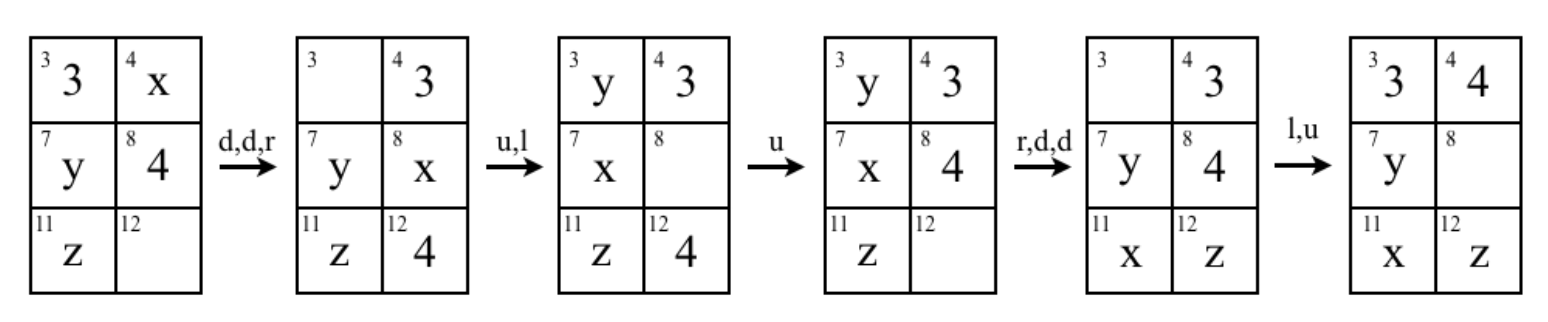
\includegraphics[width=0.8\linewidth]{movestoplace4.png}
        \caption{Mosse per portare il 4 in posizione}
        \label{fig:enter-label}
    \end{figure}
\end{itemize}
La seconda fase serve a concludere il gioco: 
\begin{itemize}
    \item ripeti la prima fase finché non sono rimaste solo due righe da sistemare; 
    \item ruota il piano di gioco di 45 gradi a destra;
    \item usa la fase uno per risolvere le nuove prime righe finché non sono rimaste solo due righe, ovvero finché non rimane un piano 2x2; 

    \begin{figure}[H]
        \centering
        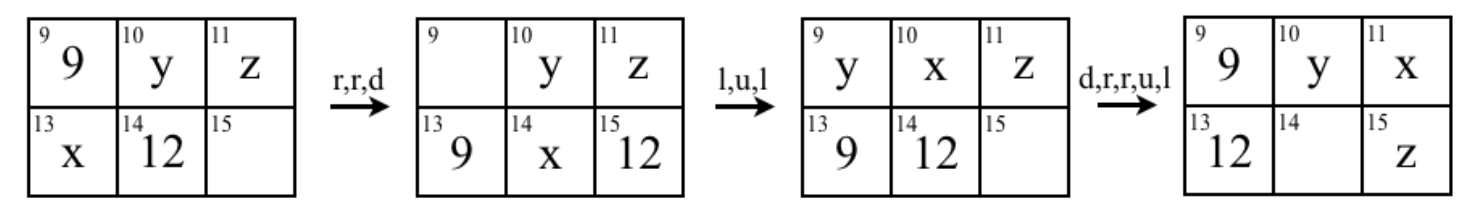
\includegraphics[width=0.8\linewidth]{mosse45gradi.png}
        \caption{seconda fase}
        \label{fig:enter-label}
    \end{figure}
    \item sposta le caselle finché il vuoto e una delle altre 3 caselle non sono in posizione corretta, le altre due dovrebbero essere automaticamente sistemate;
\end{itemize}
\chapter{Codice per la risoluzione del puzzle}
\label{codice}
\section{Introduzione}
Definiamo ora le strutture generali necessarie allo sviluppo del codice, in Java, utile allo sviluppo di un programma per la risoluzione del puzzle utilizzando i metodi introdotti nel \cref{modellazione}. 


\section{Strutture principali}
\begin{itemize}
    \item \texttt{board}: matrice intera \( N \times M \) che rappresenta lo stato attuale.
    \item \texttt{pos}: mappa che associa ogni valore alla sua posizione obiettivo.
    \item \texttt{pebbles}: mappa che associa ogni valore alla posizione corrente.
    \item \texttt{empty}: valore che identifica la cella vuota.
\end{itemize}

\subsection{Classe Board}
La seguente classe ha lo scopo di fornire una rappresentazione astratta del piano di gioco. 
La struttura è stata astratta in maniera tale che possa descrivere il gioco del 15 ma anche qualsiasi altra rappresentazione di una tavola $N \times M$. 

\begin{description}
    \item[\texttt{board}] 
        Matrice intera $N \times M$ che rappresenta lo stato attuale del puzzle, dove ogni cella contiene il valore di una tessera oppure il valore speciale della casella vuota.
        
    \item[\texttt{firstDimension}, \texttt{secondDimension}] 
        Interi che rappresentano rispettivamente il numero di righe ($N$) e di colonne ($M$) della board.
        
    \item[\texttt{empty}] 
        Valore intero che indica la tessera vuota nel puzzle (tipicamente $0$, $-1$ oppure $16$).
        
    \item[\texttt{pos}] 
        Dizionario che associa ad ogni valore di tessera la sua posizione obiettivo (riga, colonna) nella configurazione risolta del puzzle.
        
    \item[\texttt{pebbles}] 
        Dizionario che associa ad ogni valore di tessera la sua posizione attuale (riga, colonna) nella configurazione corrente.
        
    \item[\texttt{Board(int[][] tiles, int N, int M, int empty)}] 
        Costruttore della classe. Inizializza la board copiando la matrice di input, imposta le dimensioni e il valore della casella vuota, e popola i dizionari \texttt{pos} e \texttt{pebbles} per la gestione delle posizioni delle tessere.
        
    \item[\texttt{isSolvable()}] 
        Metodo che determina se la configurazione attuale del puzzle è risolvibile, calcolando il numero di inversioni e la posizione della casella vuota secondo le regole matematiche del gioco del 15.
        
    \item[\texttt{printBoard()}] 
        Stampa a video la configurazione attuale della board, utile per il debug o la visualizzazione dello stato.
        
    \item[\texttt{hamming()}] 
        Calcola e restituisce il numero di tessere fuori posto rispetto alla configurazione risolta (distanza di Hamming).
        
    \item[\texttt{manhattan()}] 
        Calcola e restituisce la somma delle distanze di Manhattan di tutte le tessere dalla loro posizione obiettivo.
        
    \item[\texttt{getPhase(int val)}] 
        Restituisce la “fase” a cui appartiene una tessera, utile per strategie di risoluzione suddivise in fasi (ad esempio, risolvere prima le righe superiori, poi le colonne, ecc.).
        
    \item[\texttt{pesoPerFase(int value, int fase)}] 
        Restituisce un peso associato a una tessera in base alla fase attuale della risoluzione, per dare priorità a certe tessere durante la ricerca.
        
    \item[\texttt{manhattanPesato(int fase)}] 
        Calcola la distanza di Manhattan pesata, cioè la somma delle distanze di tutte le tessere moltiplicata per il loro peso relativo alla fase.
        
    \item[\texttt{countLCrow(int row)}, \texttt{countLCcol(int col)}] 
        Calcolano il numero di conflitti lineari rispettivamente su una riga o su una colonna. Un conflitto lineare si verifica quando due tessere sono nella stessa riga (o colonna) della loro posizione obiettivo ma sono invertite.
        
    \item[\texttt{linearConflicts()}] 
        Calcola il numero totale di conflitti lineari su tutta la board, utile per migliorare le euristiche di ricerca.
        
    \item[\texttt{neighbors()}] 
        Genera e restituisce tutte le configurazioni adiacenti ottenibili effettuando una singola mossa (spostamento della casella vuota in una delle quattro direzioni possibili).
        
    \item[\texttt{toJSON()}] 
        Serializza la configurazione attuale della board in formato JSON, utile per esportare o salvare lo stato del puzzle.
\end{description}

\section{Possibili tecniche risolutive}
\subsection{Algoritmo A*}
Descriviamo in questa sezione le strutture utili per implementare l'algoritmo A* introdotto nel \cref{modellazione}. 

In questa implementazione l'algoritmo si basa su una disposizione iniziale del piano di gioco $N\times M$ in cui la cella vuota viene identificata dal valore $N\times M$, nel nostro caso 16. 
L'algoritmo risolutivo è quello di A* in cui vengono usate: 
\begin{itemize}
    \item una coda con proprità: per contenere a ogni iterazione le disposizioni a cui si può arrivare da quella corrente ordinate in base a una priorità in modo da scegliere sempre quella con priorità maggiore; 
    \item una lista: per contenere le disposizioni visitate finora in modo da non visitare di nuovo disposizioni visitate rischiando di rimanere bloccati in cicli infiniti; 
\end{itemize}

A ogni iterazione, quindi, l'algoritmo genera le disposizioni a cui si può arrivare da quella corrente, assegna a loro una priorità, le inserisce in una coda con priorità e sceglie la mossa successiva prendendo quella con maggiore priorità.

La priorità viene generata sommando due valori: 
\begin{itemize}
    \item numero di mosse: numero di mosse eseguite finora; 
    \item distanza di Manhattan e conflitti lineari; 
\end{itemize} I due valori rappresentano l'euristica $f(x) = g(x) + h(x)$ che guida l'algoritmo di A* nella ricerca della soluzione. Vengono quindi definite le seguenti strutture: 

\begin{description}

    \item[\texttt{Peso}] 
        Classe che contiene il parametro \texttt{peso}, usato per implementare una versione pesata dell'algoritmo A* (A* pesato). Il peso modifica l'importanza dell'euristica nella funzione di costo.

    \item[\texttt{State}] 
        Classe interna che rappresenta uno stato del puzzle durante la ricerca. Ogni oggetto \texttt{State} contiene:
        \begin{itemize}
            \item \texttt{config}: oggetto \texttt{Board} che rappresenta la configurazione attuale del puzzle.
            \item \texttt{moves}: numero di mosse effettuate per raggiungere questo stato dalla configurazione iniziale.
            \item \texttt{previous}: riferimento allo stato precedente, utile per ricostruire il percorso di soluzione.
        \end{itemize}
        Implementa l'interfaccia \texttt{Comparable} per essere inserita in una coda di priorità, confrontando gli stati in base alla funzione di priorità (tipicamente $f(n) = g(n) + h(n)$, dove $g(n)$ è il numero di mosse e $h(n)$ è una funzione euristica come la somma di Manhattan e conflitti lineari).

    \item[\texttt{astar}] 
        Classe principale che implementa l'algoritmo A* per la risoluzione del gioco del 15 (o di un puzzle $N \times M$ generico). Le sue componenti principali sono:
        \begin{itemize}
            \item \texttt{solution}: riferimento allo stato finale risolto, utile per ricostruire la soluzione;
            \item \texttt{isSolvable}: booleano che indica se la configurazione iniziale è risolvibile;
            \item \texttt{nodesExplored}: contatore dei nodi esplorati durante la ricerca;
            \item \texttt{finalConfigs}: mappa per memorizzare configurazioni finali già generate;
        \end{itemize}

    \item[\texttt{generateFinalConfig(int N, int M)}]
        Metodo che genera la configurazione finale (risolta) del puzzle, riempiendo la matrice con valori crescenti da $1$ a $N \times M$.

    \item[\texttt{astar(Board initial, int N, int M, int empty)}]
        Costruttore che esegue l'algoritmo A*, la sua implementazione è descritta dai seguenti passi:
        \begin{itemize}
            \item Genera la configurazione finale.
            \item Inizializza la coda di priorità (\texttt{openSet}) e l'insieme dei visitati (\texttt{visited}).
            \item Inserisce lo stato iniziale.
            \item Esegue il ciclo di ricerca: estrae lo stato con priorità minima, verifica se è la soluzione, esplora i vicini e aggiorna la coda.
            \item Salva la soluzione se trovata.
        \end{itemize}

    \item[\texttt{isSolvable()}]
        Restituisce \texttt{true} se la configurazione iniziale è risolvibile, altrimenti \texttt{false}.

    \item[\texttt{nodesExplored()}]
        Restituisce il numero di nodi (stati) esplorati durante la ricerca.

    \item[\texttt{moves()}]
        Restituisce il numero minimo di mosse necessarie per risolvere il puzzle, oppure $-1$ se non esiste soluzione.

    \item[\texttt{solution()}]
        Restituisce un oggetto iterabile contenente la sequenza delle configurazioni (\texttt{Board}) dalla iniziale alla finale, ricostruita a ritroso tramite i riferimenti \texttt{previous} degli stati.

    \item[\texttt{solutionToJson()}]
        Restituisce una stringa JSON che rappresenta la sequenza delle configurazioni della soluzione, utile per esportare o visualizzare la soluzione in formato strutturato.

    \item[\texttt{writeSolutionToFile(String filename, String jsonString)}]
        Scrive la soluzione in formato JSON su un file, gestendo eventuali errori di I/O.

    \item[\texttt{main(String[] args)}]
        Metodo di test che permette di eseguire l’algoritmo su una configurazione di esempio (o inserita da tastiera), stampa la soluzione, il numero di mosse e salva la soluzione in un file JSON.

\end{description}

Di seguito sono riportati alcuni degli algoritmi principali utili per l'implementazione del codice: 

\begin{algorithm}[H]
\caption{Calcolo della distanza di Manhattan nella classe \texttt{Board}}
\small
\begin{algorithmic}[1]
\Function{manhattan}{}
    \State $dist \gets 0$
    \For{$i \gets 0$ \textbf{to} $firstDimension - 1$}
        \For{$j \gets 0$ \textbf{to} $secondDimension - 1$}
            \State $value \gets board[i][j]$
            \If{$value \neq empty$}
                \State $(goalRow, goalCol) \gets pos[value]$
                \State $dist \gets dist + |i - goalRow| + |j - goalCol|$
            \EndIf
        \EndFor
    \EndFor
    \State \Return $dist$
\EndFunction
\end{algorithmic}
\end{algorithm}

\begin{algorithm}[H]
\caption{Calcolo della distanza di Manhattan pesata nella classe \texttt{Board}}
\small
\begin{algorithmic}[1]
\Function{manhattanPesato}{$fase$}
    \State $totalCost \gets 0$
    \For{$i \gets 0$ \textbf{to} $firstDimension - 1$}
        \For{$j \gets 0$ \textbf{to} $secondDimension - 1$}
            \State $value \gets board[i][j]$
            \If{$value \neq empty$}
                \State $(goalRow, goalCol) \gets pos[value]$
                \State $peso \gets$ \Call{pesoPerFase}{$value, fase$}
                \State $totalCost \gets totalCost + peso \times (|i - goalRow| + |j - goalCol|)$
            \EndIf
        \EndFor
    \EndFor
    \State \Return $totalCost$
\EndFunction
\end{algorithmic}
\end{algorithm}

\subsection{Algoritmo risolutivo}
\begin{algorithm}[H]
\caption{Algoritmo A* nella classe \texttt{astar}}
\small
\begin{algorithmic}[1]
\Function{astar}{$initial, N, M, empty$}
    \State $finalConfig \gets$ \Call{generateFinalConfig}{$N, M$}
    \State $openSet \gets$ nuova coda di priorità
    \State $visited \gets$ nuovo insieme vuoto
    \State $startState \gets$ nuovo \texttt{State} con $initial$, $moves=0$, $previous=null$
    \State inserisci $startState$ in $openSet$
    \While{$openSet$ non è vuoto}
        \State $current \gets$ estrai stato con priorità minima da $openSet$
        \If{$current.config = finalConfig$}
            \State \Return $current$ \Comment{Soluzione trovata}
        \EndIf
        \State aggiungi $current.config$ a $visited$
        \For{ogni $neighbor$ in $current.config$.neighbors()}
            \If{$neighbor$ non in $visited$}
                \State $newState \gets$ nuovo \texttt{State} con $neighbor$, $moves = current.moves + 1$, $previous = current$
                \State inserisci $newState$ in $openSet$
            \EndIf
        \EndFor
    \EndWhile
    \State \Return $null$ \Comment{Nessuna soluzione trovata}
\EndFunction
\end{algorithmic}
\end{algorithm}

\subsection{Algoritmo IDA*}
In questa sezione descriviamo le strutture utili per implementare l’algoritmo IDA*.
 
A differenza di A*, non mantiene esplicitamente l’insieme dei nodi già visitati a livello globale, ma esplora ricorsivamente i cammini fino a una soglia di costo, detta \emph{threshold}, evitando cicli tramite una lista di nodi visitati valida solo per la ricorsione corrente.  

La funzione di costo è la stessa di A*:  
\[
f(x) = g(x) + h(x)
\]  
dove $g(x)$ rappresenta la distanza di Manhattan e $h(x)$ è una funzione euristica (ad esempio il numero di mosse o i conflitti lineari).  

Il meccanismo iterativo è il seguente:  
\begin{itemize}
    \item si imposta come soglia iniziale il valore $f(x)$ della configurazione di partenza;
    \item si esegue una ricerca in profondità, visitando solo configurazioni con $f(x) \leq$ soglia;
    \item se la soluzione non viene trovata, la soglia viene aggiornata al valore minimo di $f(x)$ che ha superato la soglia corrente;
    \item si ripete il processo finché non viene trovata la soluzione o finché non esistono più nodi da esplorare.
\end{itemize}

Vengono quindi definite le seguenti strutture:  

\begin{description}

    \item[\texttt{State}]  
        Classe che rappresenta uno stato del puzzle. Contiene:
        \begin{itemize}
            \item \texttt{config}: oggetto \texttt{Board} che descrive la configurazione attuale del puzzle;
            \item \texttt{moves}: numero di mosse effettuate per raggiungere questo stato;
            \item \texttt{previous}: riferimento allo stato precedente, utile per ricostruire il percorso.
        \end{itemize}
        Definisce inoltre la funzione di priorità $f(n) = g(n) + h(n)$.

    \item[\texttt{Result}]  
        Classe interna che rappresenta l’esito di una ricerca ricorsiva. Contiene:
        \begin{itemize}
            \item \texttt{found}: indica se è stata trovata la soluzione;
            \item \texttt{nextThreshold}: la nuova soglia calcolata, da usare per l’iterazione successiva;
            \item \texttt{state}: lo stato finale se la soluzione è stata trovata.
        \end{itemize}

    \item[\texttt{idastar}]  
        Classe principale che implementa l’algoritmo IDA*. Le sue componenti principali sono:
        \begin{itemize}
            \item \texttt{solution}: riferimento allo stato finale risolto;
            \item \texttt{threshold}: soglia corrente della ricerca;
            \item \texttt{finalConfig}: configurazione finale target del puzzle.
        \end{itemize}

    \item[\texttt{idastar(Board initial)}]  
        Costruttore che avvia la ricerca IDA* a partire da una configurazione iniziale.  
        I passi principali sono:
        \begin{itemize}
            \item inizializza la soglia con il valore $f(n)$ della configurazione iniziale;
            \item esegue iterativamente la funzione \texttt{search} finché non viene trovata la soluzione o non ci sono più stati validi;
            \item aggiorna la soglia a ogni iterazione.
        \end{itemize}

    \item[\texttt{search(State current, double threshold, Set<Board> visited)}]  
        Funzione ricorsiva che esplora la configurazione \texttt{current}:
        \begin{itemize}
            \item calcola $f(n)$ e confronta con la soglia;
            \item se $f(n)$ eccede la soglia, interrompe la ricerca e aggiorna la soglia;
            \item se viene raggiunta la configurazione finale, ritorna la soluzione;
            \item esplora i vicini della configurazione corrente, evitando cicli tramite \texttt{visited};
            \item utilizza backtracking rimuovendo il nodo corrente da \texttt{visited} al termine della ricorsione.
        \end{itemize}

    \item[\texttt{moves()}]  
        Restituisce il numero di mosse della soluzione, oppure $-1$ se non esiste soluzione.

    \item[\texttt{solution()}]  
        Restituisce la sequenza di configurazioni dalla iniziale alla finale ricostruita tramite i riferimenti \texttt{previous}.

    \item[\texttt{main(String[] args)}]  
        Metodo di test: inizializza una configurazione, verifica la risolvibilità e lancia l’algoritmo IDA*, stampando a video i passi della soluzione e il numero di mosse.
\end{description}



\chapter{Teoria della complessità ~\cite{3}~\cite{4}}
\label{complessita}
\section{Alfabeti e linguaggi}
\begin{definition}
    Un simbolo è un'entità primitiva astratta, lettere e caratteri sono simboli.
\end{definition}
\begin{definition}
    Un alfabeto $\Sigma$ è un insieme finito di simboli.
\end{definition}
\begin{definition}
    Una stringa è una sequenza finita di simboli, generalmente indicata con $w$, la sua lunghezza è indicata invece con $|w|$, la stringa vuota viene indicata con $\epsilon$ ed è tale che $|\epsilon|=0$.
\end{definition}
\begin{definition}
    Un linguaggio formale è un insieme di stringhe di simboli da un alfabeto $\Sigma$. \hfill \break
    L'insieme $\emptyset$ e l'insieme $\{\epsilon\}$ sono due linguaggi formali di qualunque alfabeto. \hfill \break
    Con $\Sigma^*$ si intende un linguaggio costituito da tutte le stringhe su un fissato alfabeto $\Sigma$. 
    Ad esempio se $\Sigma=\{0\}$ allora $\Sigma^*=\{\epsilon, 0,00,000,...\}$.
\end{definition}

\section{Definizione di macchina di Turing deterministica}
Una macchina di Turing M può essere definita come una quadrupla di elementi:
$$
M = (Q, \Sigma,q_0,\delta)
$$
dove:
\begin{itemize}
    \item $Q$: insieme finito di stati;
    \item $\Sigma$: insieme finito di simboli, contiene almeno i simboli $s_0=\$$ (blank) e il simbolo $s_1 = 0$ (tally);
    \item $\delta$: funzione di transizione, dati uno stato $q$ e un simbolo di nastro $X$, $\delta(q,X)$ restituisce una tripla $(p,Y,D)$:
    \begin{itemize}
        \item $p$: è lo stato successivo; 
        \item $Y$: è il simbolo di $\Sigma$ scritto nella cella visitata; 
        \item $D$: è una direzione, può essere $L$ o $R$; 
    \end{itemize}
    \item $q_0$: lo stato iniziale;
\end{itemize}

$\delta$ può essere definito come:
$$
\delta : Q \times \Sigma \rightarrow Q \times \Sigma \times \{L,R\}
$$

Definiamo a questo punto una descrizione istantanea (ID) come una quadrupla:
$$
\langle q,v,s,w\rangle
$$
dove: 
\begin{itemize}
    \item $q \in Q$: è lo stato in cui si trova la macchina; 
    \item $v,w \in \Sigma^*$: sono i caratteri diversi da blank a sinistra e destra della testina; 
    \item $s \in \Sigma$: è il simbolo letto dalla testina;
\end{itemize}
ad esempio:
$$
X_1 X_2 ... X_{i-1} q X_i X_{i+1}...X_n
$$
in cui: 
\begin{itemize}
    \item $q$ è lo stato della macchina di Turing; 
    \item la testina visita l'i-esimo simbolo da sinistra; 
    \item $X_1X_2...X_n$ è la porzione del nastro tra il simbolo diverso dal blank più a sinistra e quello più a destra;
\end{itemize}

Otteniamo quindi che le mosse di una macchina di Turing M sono definite mediante il simbolo $\vdash_M$.

\emph{}

Supponiamo che $\delta(q,X_i)=(p,Y,L)$ cioè la prossima mossa è verso sinistra, otteniamo: 
$$
X_1X_2...X_{i-1}qX_iX_{i+1}...X_n \vdash_M X_1X_2...X_{i-2}pX_{i-1}YX_{i+1}...X_n
$$

bisogna però tenere conto di due accorgimenti: 
\begin{itemize}
    \item se $i=1$ allora la mossa a sinistra fa muovere M verso il blank, ottenendo: 
    $$
    qX_1X_2...X_n \vdash_M pBYX_2...X_n
    $$
    \item se $i=n$ e $Y=\$$ allora il simbolo $\$$ scritto su $X_n$ si unisce alla sequenza di blank e non compare nella ID: 
    $$
    X_1X_2...X_{n-1}qX_n \vdash_M X_1X_2...X_{n-2}pX_{n-1}
    $$
\end{itemize}

Ci comportiamo allo stesso modo se la testina si muove a destra. Anche in questo caso si presentano le due eccezioni precedentemente descritte cambia solo il verso nel quale si vanno a scrivere i simboli. 

Per funzionare, la stringa di input viene posta sul nastro e la testina parte dal simbolo di input più a sinistra.
Se la macchina di Turing entra in uno stato accettante allora l'input è accettato, altrimenti no.
Si ha quindi che se $M=(Q,\Sigma,q_0, \delta)$ è una macchina di Turing, allora $L(M)$ è l'insieme di stringhe $w \in \Sigma^*$ tale che $q_0w\vdash^*\alpha p\beta$ per uno stato $p$ finale e qualunque stringa di nastro $\alpha$ e $\beta$.

\section{Arresto di una macchina di Turing}
Una macchina di Turing MdT si arresta se entra in uno stato $q$ visitando un simbolo $X$ e non ci sono mosse possibili in questa situazioni.
In tal caso otteniamo che $\delta(q,X)$ è indefinito.
Possiamo sempre presumere che MdT si arresti se accetta, tuttavia, non possiamo sempre richiedere che MdT si arresti. 
I linguaggi per i quali esiste una macchina di Turing che prima o poi si arresta (indipendentemente dal fatto che accetti o no), sono detti ricorsivi. 

Invece i linguaggi che possiamo accettare usando una macchina di Turing, ma che se non accettati non ci garantiscono che la macchina si fermi, sono denominati linguaggi ricorsivamente enumerabili. 

\section{Funzioni calcolabili da MdT}
Ad ogni MdT può essere associata una funzione calcolata dalla MdT.

\begin{definition}
Assumiamo di trattare solo funzioni sui naturali e di codificare i numeri naturali in una codifica unaria in cui ogni simbolo $n\in\mathbb{N}$ è rappresentato da $n+1$ $0$ consecutivi. 
Una funzione $f:\mathbb{N}^n\rightarrow \mathbb{N}$ è Turing-calcolabile se esiste una MdT M tale che partendo dalla configurazione iniziale: 
$$
...q_0\$x_1\$...\$x_n\$...
$$
se $f(x_1,...,x_n)$ è definita allora M termina nella configurazione:
$$
...\$\$\$...q_f\$f(x_1,...,x_n)\$...
$$
altrimenti M non termina, dove per ogni $(x_1,...,x_n)\in\mathbb{N}^n$, $x_1,...,x_n$, $f(x_1,...,x_n)$ sono le rappresentazioni in unario di $x_1,...,x_n$ e $f(x_1,...,x_n)$ mentre $q_f \in Q$ è tale che per cui $\delta(q_f, \$)$ è indefinito. 
\end{definition}

\begin{definition}
Una funzione totale è una funzione definita per ogni input.
\end{definition}

\section{Macchine di Turing multinastro}
Una MdT multinastro è formata da un controllo finito e un numero $k$ finito di nastri. 
Ogni nastro è diviso in celle e ogni cella può contenere un simbolo dell'alfabeto.
L'insieme di simboli di nastro comprende un blank e ha un sottoinsieme definito di simboli di input. 
L'insieme degli stati ne comprende uno iniziale e un sottoinsieme di stati finali (accettanti). 
Una MdT multinastro inizia rispettando:
\begin{itemize}
    \item l'input si trova sul primo nastro; 
    \item tutte le altre celle contengono un blank; 
    \item il controllo si trova nello stato iniziale; 
    \item la testina del primo nastro è all'estremità sinistra dell'input; 
    \item le altre testine si trovano in celle arbitrarie siccome sono tutte blank; 
\end{itemize}

Una mossa su una MdT multinastro dipende dallo stato e dai simboli letti da ciascuna testina. 
In una mossa la macchina compie: 
\begin{itemize}
    \item il controllo entra in un nuovo stato; 
    \item su ogni cella visitata da una testina viene scritto un nuovo simbolo di nastro; 
    \item ogni testina si muove a sinistra o a destra oppure sta ferma, i movimenti sono indipendenti.
\end{itemize}

In questo caso la funzione di transazione cambia, ed è definita come: 
$$
\delta : Q \times \Sigma^k \rightarrow Q \times \Sigma^k \times \{L,R\}^k
$$
cioè è un estensione della definizione di $\delta$ per le MdT singolo nastro dove partendo da uno stato $q \in Q$ si guardano $k$ simboli (uno su ogni nastro) e restituisce una tripla formata da uno stato, $k$ simboli scritti nelle $k$ celle visitate e $k$ direzioni in cui si muovono i $k$ nastri.

\begin{theorem}
    Ogni linguaggio accettato da una MdT multinastro è ricorsivamente enumerabile.
\end{theorem}
\begin{proof}
    Sia $L$ un linguaggio accettato da una MdT con $k$ nastri, M. Simuliamo M con una MdT mononastro N il cui nastro è diviso in $2k$ tracce. 
    Metà delle tracce ($k$) replicano i nastri di M, ognuna delle restanti indica la posizione corrente della testina del corrispondente nastro di M.
\end{proof}

\section{Definizione di macchina di Turing nondeterministica}
Una macchina di Turing nondeterministica si distingue da quella deterministica in quanto la funzione $\delta$ associa a ogni stato $q$ un insieme di triple, definito come: 
$$
\delta(q,X) = \{(q_1, Y_1, D_1), (q_2, Y_2, D_2),...,(q_k,Y_k, D_k)\}
$$con $k$ intero finito. 

A ogni passo la N-MdT sceglie una delle triple come mossa.
Si ottiene che M accetta una stringa $w$ se c'è una sequenza di scelte che conduce dalla ID iniziale con $w$a una ID con stato accettante. 

\begin{theorem}
    Se $M_N$ è una macchina di Turing nondeterministica, esiste una macchina di Turing deterministica $M_D$ tale che $L(M_N)=L(M_D)$.
\end{theorem}

\section{$k-$MdT ~\cite{4}}
Una $k-$Mdt è una macchina di Turing con $k-$nastri.
Come ogni MdT è definita come $M=(Q, \Sigma, q_0, P)$ dove: 
\begin{itemize}
    \item $Q$: è l'insieme finito di stati e $q_0 \in Q$ è lo stato iniziale; 
    \item $\Sigma$: è l'alfabeto in cui assumiamo siano presenti almeno i simboli $\$$ (blank) e $\triangleright$ (first);
    \item L'insieme delle istruzioni $P$ che rappresenta una funzione di transazione $\delta$ che assumiamo essere una funzione totale: 
    $$
    \delta : Q \times \Sigma^k \rightarrow (Q \cup\{h,yes,no\})\times (\Sigma \times \{L,R,F\})^k
    $$
    \item $h,yes,no$ stati finali $\not\in Q$; 
    \item la configurazione iniziale è del tipo:
    $$
    (q_0, \underbrace{\epsilon, \triangleright, x}_{nastro \ 1}, \underbrace{\epsilon, \triangleright, \epsilon,}_{nastro \ 2}...,\underbrace{\epsilon, \triangleright, \epsilon}_{nastro \ 3})
    $$
\end{itemize}

\begin{definition}
    Una $k-$MdT è di tipo decisionale se ogni qual volta termina, raggiunge uno degli stati finali $yes$ o $no$, in questo caso l'output è lo stato raggiunto. 
    Una $k-$MdT invece calcola una funzione se ogni qual volta termina, raggiunge lo stato finale $h$, in questo caso l'output è contenuto nel nastro $h$. 
\end{definition}

\section{Classi di complessità, determinismo e nondeterminismo ~\cite{4}}
Per parlare di complessità di un determinato algoritmo, dobbiamo definire le classi di complessità, ovvero insiemi di linguaggi accumunati da una qualche proprietà.

Informalmente, quando si calcola la complessità di un determinato algoritmo, quello che si fa è andare a calcolare il tempo con il quale una macchina di Turing accetta un determinato linguaggio.

\begin{definition}
    Sia M una $k-$MdT deterministica a $k$ nastri. \hfill \break
    Sia $x$ un input della macchina. \hfill \break
    Il tempo richiesto da M per $x$ è il numero di passi di computazione necessari a $M$ con input $x$ per terminare.
\end{definition}

Il tempo però cambia nel caso in cui la macchina è una MdT deterministica oppure non. 

\begin{definition}
    Sia $f: \mathbb{N} \rightarrow \mathbb{N}$ una funzione totale. \hfill \break
    Sia M una $k-$MdT deterministica a $k$ nastri. \hfill \break
    Sia $x$ un input della macchina. \hfill \break
    Una $k-$MdT opera in tempo $f(n)$ se per ogni input $x$ il tempo richiesto da $M$ per $x$ è minore o uguale a $f(|x|)$, supponendo che $|x|=n$ questo vuol dire minore o uguale a $f(n)$. 
\end{definition}

Un linguaggio $L\subseteq\Sigma^*$ è deciso da una k-MdT M:
\begin{itemize}
    \item se $x\in L$ allora $M(x)=yes$;
    \item se $x\not\in L$ allora $M(x)=no$;
\end{itemize}

\begin{definition}
    Se $L \subseteq \Sigma^*$ è deciso da una k-MdT M e M opera in tempo $f(n)$, allora $L\in TIME(f(n))$, quindi $TIME(f(n))$ è una classe di complessità in tempo. 
\end{definition}

\begin{definition}
    Un linguaggio $L \subseteq \Sigma^*$ è deciso da una MdT non deterministica M se per ogni $x \in \Sigma^*$: 
    \begin{itemize}
        \item se $x \in L$ allora esiste una computazione nondeterministica tale che: 
        $$
        (q_0, \epsilon, \triangleright, x) \rightarrow_* (yes, u,s,v)
        $$
        \item se $x \not\in L$ allora non esiste una computazione non deterministica tale che: 
        $$
        (q_0, \epsilon, \triangleright, x) \rightarrow_* (yes, u,s,v)
        $$
    \end{itemize}
\end{definition}

\begin{definition}
    Una ND-MdT M opera in tempo $f(n)$ se per ogni $x \in \Sigma^*$, ogni computazione non deterministica sull'input $x$ ha al più lunghezza $f(|x|)$.
\end{definition}

Quindi nel caso di ND-MdT non è l'intera macchina a operare in tempo $f(n)$ ma ogni ramo della computazione non deterministica. 

\begin{figure}[H]
    \centering
    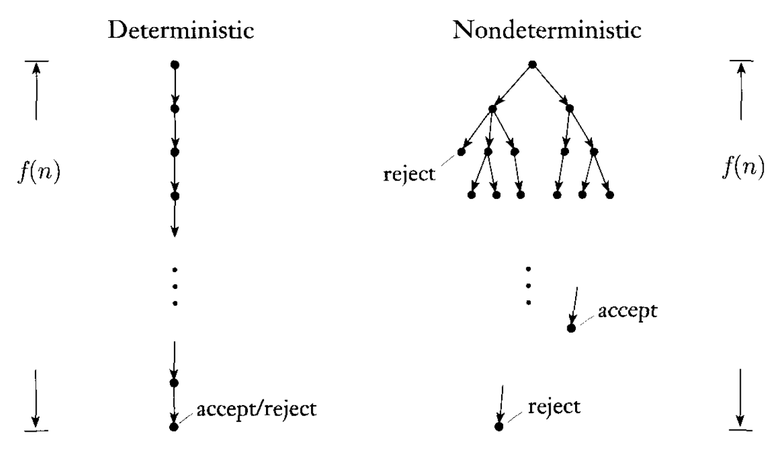
\includegraphics[width=0.5\linewidth]{Mdt e NMdt.png}
    \caption{Differenza tra MdT deterministica e non}
    \label{fig:enter-label}
\end{figure}

\begin{definition}
    Se un linguaggio $L\in \Sigma^*$ è deciso da una N-MdT M che opera in tempo $f(n)$ allora $L\in NTIME(f(n))$. 
\end{definition}

\section{Classe di complessità P ~\cite{5}} 
\begin{definition}
    La classe di complessità P è l'insieme di tutti i linguaggi che possono essere decisi in tempo polinomiale, ovvero:
    $$
    P = \bigcup_k \ TIME(n^k)
    $$
\end{definition}

\section{Classe di complessità NP \cite{5}}
\begin{definition}
    La classe di complessità NP è l'insieme di tutti i linguaggi che possono essere decisi in tempo polinomiale da una macchina non deterministica, ovvero:
    $$
    NP = \bigcup_k \ NTIME(n^k)
    $$
\end{definition}

\section{Riduzioni polinomiali}
La tecnica per dimostrare che un problema $P_2$ non può essere risolto in tempo polinomiale è la riduzione di un problema $P_1$, che si sa non essere $\mathcal{P}$, a $P_2$. 
Bisogna, però, richiedere un ulteriore vincolo: la traduzione da $P_1$ a $P_2$ deve richiedere un tempo polinomiale nella lunghezza dell'input.
 
\section{Problemi NP-completi e NP-hard}
\begin{definition}
    Diciamo che $L$ è $NP-$completo se:
    \begin{itemize}
        \item $L$ è in $NP$;
        \item per ogni linguaggio $L'$ in $NP$ esiste una riduzione polinomiale di $L'$ a $L$;
    \end{itemize}
\end{definition}

Su alcuni problemi $L$, sebbene sia possibile dimostrare la seconda condizione non è possibile dimostrare la prima, ovvero che $L\in NP$, tali problemi prendono il nome di NP-hard. 

\section{Il problema SAT}
Il problema di soddisfacibilità booleana, detto più comunemente SAT, è un esempio di problema NP-completo. 
\hfill \break
Il problema si basa sull'andare a decidere se un'espressione booleana è soddisfacibile. 

\hfill \break 
Le espressioni booleane sono formate da: 
\begin{itemize}
    \item variabili a valori booleani ovvero 1 per indicare true e 0 per indicare false; 
    \item gli operatori binari $\land$ e $\lor$ per indicare rispettivamente AND e OR;
    \item l'operatore unario $\lnot$ che indica la negazione logica; 
    \item parentesi per raggruppare il tutto; 
\end{itemize}

\begin{example}
    Un esempio di espressione booleana è $x \land \lnot(y \lor z)$.
\end{example}

\begin{definition}
    Un assegnamento di valori di verità per un espressione booleana E assegna i valori vero o falso a ognuna delle variabili presenti in E, di conseguenza il valore dell'espressione E a seguito dell'assegnamento T è indicato con $E(T)$.
    Se $E(T)=1$ allora l'espressione è soddisfatta, senò no.
\end{definition}

\noindent Il problema della soddisfacibilità è definito come:
 \begin{itemize}
     \item un'espressione booleana assegnata è soddisfacibile?
 \end{itemize}

Enunciato come linguaggio, SAT è l'insieme delle espressioni booleane soddisfacibili. 

Bisogna però trovare un modo per codificare il SAT. 
In un espressione booleana possono esserci un numero infinito di simboli, bisogna ideare un codice con un alfabeto finito per rappresentare espressioni che possono essere infinitamente grandi. 
Per farlo: 
\begin{itemize}
    \item rappresentiamo gli operatori binari e unari da se stessi ($\lnot, \land,\lor$);
    \item rappresentiamo la variabile $x_i$ come $x$ seguito dalla codifica binaria di $i$;
\end{itemize}

\begin{example}
    Ad esempio $\lnot x_1\land (x_2\lor x_3)$ equivale a $\lnot x1 \land(x10\lor x11)$ 
\end{example}

\subsection{NP-completezza del problema SAT}
Per dimostrare la NP-completezza di SAT andiamo a usare la riduzione per ridurre un qualsiasi linguaggio NP (accettato da un N-MdT in tempo polinomiale) a SAT. Per provare che SAT è NP-completo bisogna provare che: 

\begin{enumerate}
    \item SAT sta in NP;
    \item qualsiasi altro linguaggio in NP è riducibile a SAT; 
\end{enumerate}

\begin{proof}
Dimostriamo che SAT è NP-completo: 
    \begin{enumerate}
        \item Per provare che SAT è NP sfruttiamo una N-MdT. Supponiamo di avere un espressione booleana E e una macchina di Turing non deterministica M. Costruiamo M in modo tale che grazie al non determinismo provi tutti gli assegnamenti possibili di valori di verità in E. Ogni diramazione rappresenta quindi il tentativo di un diverso assegnamento di valori. Si possono raggiungere $2^n$ ID, ovvero configurazioni diverse e a questo punto basta valutare E per l'assegnamento di valori fatto (in ogni diramazione), se $E(T)=1$ allora accettiamo. Una N-MdT multinastro effettua la valutazione in tempo $O(n^2)$ mentre una singolo nastro in tempo $O(n^4)$, che è comunque polinomiale. 
        \item Sia $L$ un linguaggio qualsiasi appartenente a NP. Per definizione, esiste una macchina di Turing non deterministica $M$ che decide $L$ in tempo polinomiale $p(n)$. L'idea della riduzione è costruire, a partire da un'istanza $x$ di $L$, una formula booleana $\varphi_x$ tale che:\[\varphi_x \text{ è soddisfacibile } \iff x \in L.\] La costruzione avviene codificando il calcolo di $M$ su input $x$ in una tabella \textit{tempo × spazio}, dove ogni cella rappresenta il contenuto di un nastro, lo stato della macchina e la posizione della testina in un determinato passo. Le condizioni di correttezza del calcolo (transizioni valide, stato iniziale corretto, stato finale accettante) vengono espresse tramite vincoli booleani. La formula risultante $\varphi_x$ ha dimensione polinomiale rispetto a $|x|$ e può essere costruita in tempo polinomiale. Pertanto, ogni problema in NP si riduce in tempo polinomiale a SAT. ~\cite{7}
    \end{enumerate}
\end{proof}

\subsection{Variante di SAT: 3SAT}
Una versione ristretta del problema SAT molto utilizzata in Informatica è la variante 3SAT. 
Anche questo è un problema di soddisfacibilità booleana ma dove le espressioni booleane sono congiunzioni di disgiunzioni di esattamente tre variabili. 
Formalmente il 3SAT prende in input istanze di SAT in cui ogni clausola consta di esattamente 3 elementi e si pone come problema quello di stabilire, come per SAT, se esiste un assegnamento che rende vera la formula. 


\begin{example}
    Un esempio di espressione $E$ che rispetta le ipotesi di 3SAT è $(x_1 \lor x_2 \lor \lnot x_3) \land (\lnot x_1 \lor x_2 \lor x_3$). 
\end{example}

\begin{theorem}
    3SAT, come SAT, è NP-completo. 
\end{theorem}
\begin{proof}
    L'appartenenza a NP si mostra in quanto ogni istanza di 3SAT è anche istanza di SAT.
    Abbiamo già dimostrato che ogni problema in NP si può ridurre a SAT, mostriamo che ogni problema NP si può ridurre a 3SAT mostrando che SAT si può ridurre a 3SAT (SAT $\preceq$ 3SAT).
    Per farlo ci basta tradurre ogni clausola $l_1\lor...\lor l_m$ in una clausola uguale di 3SAT:
    \begin{itemize}
        \item se m=1: la trasformo in $l_1 \lor l_1 \lor l_1$;
        \item se m=2: la trasformo in $l_1 \lor l_2 \lor l_2$;
        \item se m=3: la tengo così com'è; 
        \item se m$>$3: introduco una nuova variabile X e restituisco $l_1 \lor l_2 \lor X$ e $\lnot X \lor l_4 \lor ... \lor l_m$ e riapplico la regola;
    \end{itemize}
\end{proof}

\section{3-Dimensional Matching (3DM) ~\cite{6}} 
Dati 3 insiemi disgiunti X,Y,Z di uguale dimensione $n$.
Dato un insieme di triple $T\subseteq X \times Y \times Z$.
Esiste un sottoinsieme $S\subseteq T$ tale che ogni elemento $\in X \cup Y \cup Z$ è in esattamente una tripla $s \in S$. 

\begin{theorem}
    3DM è NP-completo.
\end{theorem}
\begin{proof}
    Per dimostrare la NP-completezza di 3DM dobbiamo dimostrare sia che 3DM appartiene a NP, sia che ogni problema in NP è riducibile a 3DM. 
    La seconda parte la dimostriamo dimostrando che 3SAT è riducibile a 3DM e siccome abbiamo già dimostrato che SAT è riducibile a 3SAT e SAT soddisfa l'ipotesi, allora anche 3DM la soddisfa. 
    \begin{itemize}
        \item per dimostrare che 3DM appartiene a NP basta considerare un algoritmo non deterministico che crea un sottoinsieme di triple e in tempo polinomiale verifica che nessuna delle triple sia intersecata;
        \item riduciamo 3SAT a 3DM. Sia $U=\{u_1,u_2,...,u_n\}$ l'insieme delle variabili e sia $C=\{c_1,c_2,...,c_m\}$ l'insieme delle clausole.
        Cerchiamo di costruire 3 insiemi disgiunti $X,Y,Z$ e un insieme $M \subseteq X \times Y \times Z$ tale che M contenga una tripla se e solo se tutte le clausole di $C$ sono soddisfacibili.
        L'insieme delle triple M può essere visto come partizionato in 3 parti che possiamo definire variable gadget, clause gadget e garbage collection. La prima componente corrisponde alle singole variabili $u\in U$, per ognuna di esse vengono creati due elementi $y_{u_i}\in Y$ e $z_{u_i} \in Z$ che vanno a creare una tripla insieme a $u_i$. In questo caso si veranno a creare $2nu_i$ triple dove $nu_i$ rappresenta il numero di clausole in cui è presente la variabile $u_i$. Il tutto può essere rappresentato attraverso un grafo sul quale veranno mappate le variabili $u_i$ e le loro negazioni $\lnot u_i$, si ottiene una situazione rappresentabile come: 
        \begin{figure}[H]
            \centering
            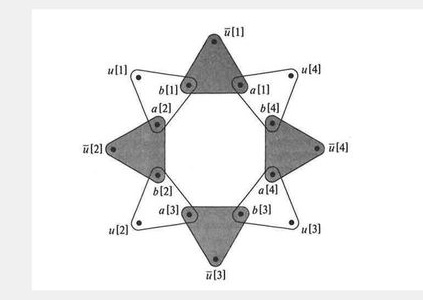
\includegraphics[width=0.5\linewidth]{variablegadget.jpeg}
            \caption{Truth setting component o variable gadget}
            \label{fig:enter-label}
        \end{figure}
        Si ottengono in questo modo due insiemi: 
        $$
        %\begin{align}
        T_i^t = \{(\lnot u_i, y_{u_i}, z_{u_i})\} \\
        T_i^f = \{(u_i, y_{u_i}, z_{u_{i+1}})\} \\
        %\end{align}
        $$
        $$
        T = T_i^f \cup T_i^t
        $$
        Si nota quindi che in ogni caso, per non sovrapporre gli elementi, si dovranno scegliere o i triangoli che contengono il valore positivo $u_i$ o la sua negazione, questo obbliga a scegliere un valore di verità per una delle variabili. 
        Allo stesso modo si crea la variable gadget, dove ogni variabile forma una tripla con due nuove variabili $y_c, z_c$ per ogni clausola $c_j \in C$ presente in $E$, questo per indicare quali variabili appaiono in quali clausole, si forma quindi: 
        $$
        C_j = \{(u_{ij},y_{c_j}, z_{c_j}): u_i \in c_j\} \cup \{(\lnot u_{ij},y_{c_j}, z_{c_j}): u_i \in c_j\}
        $$
        Per completare la costruzione viene usata la garbage collection che unisce ogni variabile ($u_i$) e la sua negazione ($\lnot u_i$) a due componenti $y_{g_k}\in Y$ e $z_{g_k}\in Z$, in questo modo tutti gli elementi che non appaiono in variable gadget o in clause gadget possono essere recuperate sfruttando la garbage collection: 
        $$
        G = \{(u_{ij},y_{g_k}, z_{g_k}), (\lnot u_{ij}, y_{g_k}, z_{g_k})\}
        $$
        Infine, creando un insieme di triple in modo che ogni elemento di $X \times Y \times Z$ appaia esattamente in una sola tripla:
        $$
        M = (\bigcup_{i=1}^{n}T_i) \cup (\bigcup_{j=1}^mC_j) \cup G
        $$
        abbiamo ridotto il problema di SAT a 3DM. 
    \end{itemize}
\end{proof}

\section{3-Exact-Cover (X3C)}
Sia $X$ un insieme finito con $|X|=3q$ elementi e una collezione $C$ di sottoinsiemi di 3 elementi di $X$ ci chiediamo se $C$ contiene una exact cover per X, cioè, se esiste una collezione $C' \subseteq C$ tale che ogni elemento di $X$ appare esattamente una volta in $C'$.

Si noti che 3DM non è altro che una versione ristretta di X3C.

Infatti è possibile ridurre il problema del 3DM a 3XC.

Sia $C = \{\{x,y,z\}: (x,y,z) \in T\}$ e sia $k = |X| =|Y|=|Z|=n$. 
Otteniamo che $C$ è una collezione di sottoinsiemi di $T$ dove $T$ è l'insieme delle triple di valori e $k$ rappresenta il numero di sottoinsiemi di $C$, ovvero $|C'|=k$, cioè ogni tripla rappresenta un sottoinsieme di $C$, ciò che vogliamo è che ogni elemento di $C'$ sia una tripla disgiunta. 
Supponiamo $M$ sia la soluzione al 3DM. 
Sia $C' = \{\{x,y,z\}: (x,y,z)\in M\}$, abbiamo $|M|=n=|C'|$. 
Sappiamo che se $(x,y,z)$ e $(x',y',z')$ sono due elementi distinti di $M$ allora, siccome per definizione $X\cap Y \cap Z = \emptyset$ avremmo $\{x,y,z\} \cap \{x',y',z\} = \emptyset$. 
Cioè gli elementi in $C'$ sono a due a due disgiunti, e siccome coprono tutti gli elementi dell'insieme universo, otteniamo che $C'$ è una soluzione al 3XC. 

Allo stesso modo, supponiamo $C'=\{C_1,C_2,...,C_k\}$ sia una soluzione al 3XC.
Sia $M=\{(x,y,z): \{x,y,z\} = C_i \ per \ i = 1,2,...k \}$.
Siccome gli $C_i'$ sono a due a due disgiunti, se $(x,y,z)$ e $(x',y',z')$ sono due elementi distinti di $M$ allora sono tutti distinti. 
Quindi $M$ è una soluzione al 3DM. 

Avendo quindi dimostrato che 3DM è un problema NP-completo, si dimostra che anche X3C lo è. 


\chapter{Dimostrazione della NP-completezza della ricerca della sequenza di mosse minore per passare da una configurazione a un altra nel gioco del 15}
 In principio il problema di calcolare la minor sequenza di mosse che servono per passare da una configurazione del gioco del 15 a un altra è stato dimostrato, da parte di Oded Goldreich, essere un problema NP-hard.
 Nella sua dimostrazione Goldreich dimostra tale assunto riducendo il problema di 3-Exact-Cover (3XC), descritto sopra, a una formalizzazione del problema del gioco del 15. ~\cite{2}

La dimostrazione però può essere fatta anche in un secondo modo ovvero considerando i concetti di gruppo e generatore.

\section{Definizione di gruppo}
Un gruppo è una struttura algebrica $(G, \cdot)$ costituita da un insieme $G$ non vuoto munito di un'operazione binaria $\cdot : G \times G \to G$ che soddisfa i seguenti assiomi:
\begin{itemize}
    \item Associatività: Per ogni $a, b, c \in G$, si ha $(a \cdot b) \cdot c = a \cdot (b \cdot c)$
    \item Elemento neutro: Esiste un elemento $e \in G$ tale che per ogni $a \in G$, $e \cdot a = a \cdot e = a$
    \item Elemento inverso: Per ogni $a \in G$, esiste un elemento $a^{-1} \in G$ tale che $a \cdot a^{-1} = a^{-1} \cdot a = e$
\end{itemize}

Nel contesto delle permutazioni, i gruppi emergono dal fatto che ogni permutazione di un insieme finito $X = {1, 2, \ldots, n}$ può essere vista come una funzione biiettiva $\sigma: X \to X$. L'insieme di tutte le permutazioni di $X$, denotato $S_n$, forma un gruppo rispetto alla composizione di funzioni, chiamato gruppo simmetrico di grado $n$.

\section{Generatori di un gruppo}
Sia $(G, \cdot)$ un gruppo e sia $S \subseteq G$ un sottoinsieme. Il sottogruppo generato da $S$, denotato $\langle S \rangle$, è il più piccolo sottogruppo di $G$ che contiene tutti gli elementi di $S$.
Equivalentemente, $\langle S \rangle$ è l'insieme di tutti gli elementi di $G$ che possono essere espressi come prodotto finito di elementi di $S$ e dei loro inversi.

Un sottoinsieme $S \subseteq G$ si dice insieme di generatori di $G$ se $\langle S \rangle = G$, ovvero se ogni elemento di $G$ può essere espresso come combinazione finita di elementi di $S$ e dei loro inversi.

\section{Gruppi, permutazioni e gioco del 15}
Nel nostro caso possiamo formalizzare il gioco del 15 con un gruppo.
Consideriamo: 
\begin{itemize}
    \item un insieme di elementi: nel nostro caso i numeri da 1 a 16;
    \item i generatori come qualsiasi trasposizione di una pedina con la cella vuota (16); 
\end{itemize}

\section{Ricerca del numero minimo di mosse per passare da una permutazione a un altra e teoria dei gruppi}

Il motivo per cui siamo interessati ai gruppi e alla teoria dei gruppi è perché la ricerca del numero minore di mosse che portano da una configurazione del piano di gioco alla soluzione corrisponde al problema di trovare la più breve sequenza generatrice che realizza una permutazione. ~\cite{2} 

Problema che è stato dimostrato essere NP-hard. ~\cite{9} 
Essendo ogni generatore una trasposizione tra una pedina e la cella vuota, questo equivale a cercare il numero minimo di trasposizioni che portano alla soluzione.
Ma essendo ogni trasposizione (mossa) rappresentabile con una permutazione questo equivale a cercare il numero minimo di permutazioni del piano di gioco che portano alla soluzione. 

\section{Grafi di Cayley e problema del calcolo del diametro}
Il nostro problema può essere dimostrato essere NP-hard seguendo anche una seconda strada, ovvero sfruttando il concetto di grafo di Cayley. 

Un grafo di Cayley è una struttura matematica che fornisce una rappresentazione geometrica di un gruppo attraverso la teoria dei grafi. Formalmente, dato un gruppo finito $G$ e un insieme di generatori $S \subseteq G$ tale che $S$ non contenga l'elemento neutro e sia chiuso rispetto all'inverso, il grafo di Cayley contiene un vertice che corrisponde a ogni elemento del gruppo $G$ e un arco tra due vertici $g$ e $h$ se esiste un generatore $s \in S$ tale che $h$ può essere ottenuto da $g$ moltiplicando per $s$. 

Nel nostro caso ogni vertice del grafo corrisponde a una configurazione del puzzle.
Ogni arco collega due configurazioni se è possibile passare dall’una all’altra tramite una mossa elementare.
Così, il grafo di Cayley rappresenta tutte le possibili disposizioni e le transizioni tra di esse.

Il diametro di un grafo connesso $G$ è la massima distanza tra due vertici qualsiasi del grafo:
\[
\text{diam}(G) = \max_{u,v \in V(G)} d(u,v)
\]
dove $d(u,v)$ denota la lunghezza del cammino più breve tra $u$ e $v$.

Nel contesto dei grafi di Cayley, il diametro ha un'interpretazione algebrica particolarmente significativa: rappresenta il numero minimo di elementi dell'insieme generatore $S$ necessari per esprimere qualsiasi elemento del gruppo come prodotto di generatori. Nel puzzle del 15, il diametro del grafo di Cayley corrisponde al numero massimo di mosse minime necessarie per risolvere qualsiasi configurazione. 

Calcolare il diametro di un grafo di Cayley è stato più volte dimostrato essere un problema NP-hard. ~\cite{10}

\chapter{Calcolo delle complessità computazionali degli pseudocodici proposti}
Analizziamo ora dal punto di vista della complessità computazionale gli algoritmi che sono stati proposti (\cref{codice}) per affrontare la risoluzione del gioco del 15. L’obiettivo è valutare, per ciascun approccio, l’ordine di grandezza del tempo di esecuzione e dello spazio in memoria richiesto.

\section{Calcolo dell'esistenza del routing number}
Come già descritto nel \cref{routing number}, l'algoritmo descritto ha una complessità temporale che dipende dalla struttura del grafo e dal numero di nodi $n$. In particolare:

\begin{itemize}
    \item Il calcolo che coinvolge una BFS per ogni nodo, ha una complessità di $O(n + m)$, dove $n$ è il numero di nodi e $m$ il numero di archi nel grafo.
    \item In generale, il numero massimo di passi necessari è di $O(n+m)$;
\end{itemize}

Pertanto, la complessità complessiva dell'algoritmo è $O(n+m)$.

\section{Algoritmo di verifica di risolvibilità}
Anche questo algoritmo è già stato analizzato all'interno del \cref{modellazione}. Ribadiamo che a causa del doppio ciclo for utilizzato per contare le inversioni l'algoritmo ha una complessità pari a $O(n^2)$. 

\section{Algoritmo risolutivo: A*}
La complessità temporale di A* è espressa in funzione di due parametri fondamentali:\begin{itemize}
    \item \textbf{$b$}: fattore di branching (numero medio di successori per nodo);
    \item \textbf{$d$}: profondità della soluzione ottima;
\end{itemize}
Nel caso peggiore, A* presenta una complessità temporale di $\mathcal{O}(b^d)$, equivalente a quella di una ricerca in ampiezza. Tuttavia, questa rappresenta uno scenario che raramente si verifica.

In generale A* ha una complessità: 
\begin{itemize} 
    \item \textbf{Caso migliore}: quando l'euristica è perfetta A* esplora solo i nodi lungo il percorso ottimo, risultando in una complessità temporale $\mathcal{O}(d)$.
    \item \textbf{Caso peggiore}: A* degenera in una ricerca con complessità $\mathcal{O}(b^d)$ equivalente a una in ampiezza;
    \item \textbf{Caso medio}: con euristiche ammissibili la complessità si riduce rispetto al caso peggiore nell'ordine di $\mathcal{O}(b^{d \cdot \varepsilon})$ dove $\varepsilon < 1$ dipende dalla qualità dell'euristica.
\end{itemize}

La complessità di A* dipende quindi fortemente dall'euristica che viene utilizzata. 

\subsection{Analisi della Complessità nell'Implementazione}
Nel codice implementato per il gioco del 15 il fattore di branching è limitato a 4 (movimenti nelle quattro direzioni).

Nell'implementazione però vengono usati vari metodi per "filtrare" la ricerca.
Il seguente frammento di codice illustra la generazione e il filtraggio dei nodi successori:

\begin{lstlisting}[language=Java, caption=Generazione dei nodi successori]
for (Board neighbor : neighborsList) {
    if (!visited.contains(neighbor)) {
        visited.add(neighbor);
        openSet.add(new State(neighbor, current.moves + 1, current));
    }
}
\end{lstlisting}

Il fattore di branching viene in questo modo ridotto in quanto:
\begin{enumerate}
    \item la tessera vuota può avere 2, 3 o 4 movimenti possibili a seconda della posizione;
    \item l'utilizzo del \texttt{Set<Board> visited} elimina la rivisitazione degli stati;
\end{enumerate}

La funzione di priorità implementata segue la formulazione classica di A*:
$$f(n) = g(n) + h(n)$$

dove $g(n)$ rappresenta il costo del percorso dalla radice al nodo $n$, e $h(n)$ è la stima euristica del costo dal nodo $n$ alla soluzione.

\begin{lstlisting}[language=Java, caption=Implementazione della funzione di priorità]
public int priority() {
    return this.moves + config.manhattan();
}
\end{lstlisting}

L'euristica combinata utilizza:
\begin{itemize}
    \item \textbf{Distanza di Manhattan}: $\mathcal{O}(1)$ calcola la distanza di ogni pedina dalla posizione "obiettivo"; 
    \item \textbf{Numero di mosse}: $\mathcal{O}(n)$ il numero esatto di mosse dalla configurazione iniziale
\end{itemize}

\begin{lstlisting}[language=Java, caption=Calcolo delle distanze di Manhattan]
        public int manhattan() {
        int dist = 0;
        for (int i = 0; i < this.firstDimension; i++) {
            for (int j = 0; j < this.secondDimension; j++) {
                int value = board[i][j];
                if (value != empty) {
                    Pair targetPosition = pos.get(value); 
                    dist += Math.abs(i - targetPosition.first) + Math.abs(j - targetPosition.second);

                }
            }
        }
        return dist;
    }
\end{lstlisting}

La distanza di Manhattan ha complessità computazionale $O(N^2)$ per puzzle $N×N$ in quanto, in questo caso, il calcolo viene svolto ogni volta, cioè non viene utilizzata alcuna tecnica di memoizzazione. 
Nel caso di utilizzo di memoizzazione tale complessità è riducibile al valore di $O(1)$.


Il codice include una verifica preliminare che previene calcoli inutili nel caso di disposizioni che non sono risolvibili. 
La complessità di questo codice è già stata trattata ed è nell'ordine di $O(n^2)$.


Questa ottimizzazione elimina a priori le configurazioni non risolvibili, evitando esplorazioni infinite dello spazio degli stati.


L'implementazione utilizza strutture dati ottimizzate per le operazioni critiche:
\begin{lstlisting}[language=Java, caption=Inizializzazione delle strutture dati]
PriorityQueue<State> openSet = new PriorityQueue<>();
Set<Board> visited = new HashSet<>();
\end{lstlisting}
Le complessità delle operazioni fondamentali sono:
\begin{itemize}
    \item \textbf{PriorityQueue.poll()}: $O(logn)$ per l'estrazione del nodo con priorità minima;
    \item \textbf{HashSet.contains()}: $O(1)$ medio per la verifica di appartenenza;
    \item \textbf{PriorityQueue.add()}: $O(logn)$ per l'inserimento ordinato;
\end{itemize}

Il confronto tra stati è implementato direttamente nella classe \texttt{State}:
\begin{lstlisting}[language=Java, caption=Implementazione del comparatore, float=h]
@Override
public int compareTo(State y) {
if (this.priority() > y.priority()) {
return 1;
} else if (this.priority() < y.priority()) {
return -1;
} else {
return 0;
}
}
\end{lstlisting}
Questa implementazione garantisce un ordinamento corretto degli stati nella coda di priorità, fondamentale per il funzionamento ottimale di A*.

La distanza di Manhattan, pur essendo ammissibile, presenta una limitazione:
\begin{itemize}
    \item \textbf{Non considera i conflitti}: tessere che si bloccano reciprocamente non sono rilevate
\end{itemize}

Questa può portare a un aumento del numero di nodi esplorati rispetto a euristiche più informative come quella che combina Manhattan e conflitti lineari.

L'algoritmo A* implementato con la distanza di Manhattan come euristica presenta una complessità temporale teorica $O(b^d)$ con prestazioni che dipendono fortemente dalla qualità dell'euristica.

\subsection{Algoritmo: A* con conflitti lineari}

La versione dell'algoritmo A* implementata considera, oltre alla distanza di Manhattan, anche i \emph{conflitti lineari} come parte dell'euristica. Questa scelta consente di rendere l'euristica più informativa e ridurre il numero di nodi esplorati.

\begin{itemize}
    \item La funzione di priorità $f(n)$ viene calcolata come:
    \[
        f(n) = g(n) + h(n) = \text{\#mosse dalla radice} + (\text{distanza di Manhattan} + \text{conflitti lineari})
    \]I conflitti lineari permettono di rilevare situazioni in cui due o più tessere si bloccano reciprocamente sulla stessa riga o colonna, aumentando il valore dell'euristica in modo da scoraggiare percorsi non ottimali.

    \item La classe \texttt{State} è stata aggiornata affinché il metodo \texttt{priority()} includa il calcolo dei conflitti lineari:
\begin{lstlisting}[language=Java]
public int priority() {
    return config.linearConflicts() + config.manhattan();
}
\end{lstlisting}
    \item La struttura dei nodi successori e la gestione della coda di priorità rimangono identiche, ma la combinazione di Manhattan e conflitti lineari migliora la selezione del nodo successivo da esplorare.
\end{itemize}

\begin{itemize}
    \item L'aggiunta dei conflitti lineari aumenta il costo computazionale per il calcolo dell'euristica di ciascun nodo. Il numero totale di nodi esplorati diminuisce sensibilmente rispetto all'uso della sola distanza di Manhattan.
    \item La complessità temporale rimane $\mathcal{O}(b^d)$ nel caso peggiore, ma nella pratica il fattore di branching effettivo viene ridotto grazie alla guida più precisa.
    \item L'implementazione continua a utilizzare un \texttt{HashSet} per i nodi visitati, evitando di riesplorare stati già considerati durante la ricerca.
\end{itemize}
Questa versione dell'algoritmo permette di ottenere soluzioni più rapide e vicine al numero minimo di mosse rispetto all'A* basato solo sulla distanza di Manhattan, grazie alla maggiore precisione dell'euristica combinata.

\section{Algoritmo risolutivo: IDA*}

L'algoritmo IDA* (Iterative Deepening A*) è una variante dell'A* che combina la profondità limitata tipica della DFS con l'euristica di A*. A differenza di A*, IDA* utilizza una soglia (threshold) per guidare la ricerca in profondità, evitando di memorizzare tutti i nodi esplorati e riducendo significativamente l'uso della memoria.
\begin{itemize}
    \item La funzione di costo $f(n) = g(n) + h(n)$ è calcolata esattamente come in A*, dove $g(n)$ è il numero di mosse dalla radice e $h(n)$ è l'euristica (somma di Manhattan e conflitti lineari, se implementata).
    \item La soglia iniziale viene impostata al costo del nodo iniziale $f(start)$.
    \item L'algoritmo esegue una ricerca in profondità limitata dalla soglia. Se un nodo supera la soglia, viene ignorato, ma viene registrato il minimo $f$ oltre la soglia per aggiornare la soglia nella prossima iterazione.
    \item La lista \texttt{visited} serve solo per evitare cicli all'interno della stessa iterazione ricorsiva, consentendo però di riesplorare gli stessi nodi in iterazioni successive.
\end{itemize}
L'implementazione utilizza:
\begin{itemize}
    \item Una classe \texttt{State} che rappresenta ciascun stato del puzzle, memorizzando la configurazione, il numero di mosse e il nodo precedente per ricostruire il percorso.
    \item Un metodo ricorsivo \texttt{search} che esplora i vicini di ciascuno stato secondo la logica DFS e confronta $f(n)$ con la soglia corrente.
    \item La soglia viene aggiornata a ogni iterazione con il minimo $f(n)$ dei nodi che l'hanno superata, permettendo di approfondire gradualmente lo spazio degli stati.
\end{itemize}

Nel calcolo della complessità IDA* si distingue principalmente per l'uso della memoria che fa: 

\begin{itemize}
    \item \textbf{Memoria:} $O(d)$, dove $d$ è la profondità massima della soluzione. L'algoritmo memorizza solo il percorso corrente nella ricorsione, evitando di salvare tutti i nodi visitati come fa A*.
    \item \textbf{Tempo:} nel caso peggiore, IDA* può visitare ripetutamente gli stessi nodi in iterazioni successive. La complessità temporale è quindi $O(b^d)$, simile a quella di A*, ma con un fattore moltiplicativo dovuto alle ripetizioni dovute all’approccio iterativo.
    \item L'uso della lista \texttt{visited} locale riduce i cicli durante la DFS, ma non elimina completamente le riesplorazioni tra iterazioni successive.
\end{itemize}

IDA* richiede quindi molta meno memoria, in quanto non mantiene tutti i nodi esplorati in una coda di priorità globale.

\section{Tabella riassuntiva}
\begin{table}[h!]
\centering
\caption{Confronto tra A*, A* con conflitti lineari e IDA* per il gioco del 15}
\resizebox{\textwidth}{!}{%
\begin{tabular}{|l|p{4cm}|p{4cm}|p{4cm}|}
\hline
\textbf{Caratteristica} & \textbf{A*} & \textbf{A* con conflitti lineari} & \textbf{IDA*} \\
\hline
Strategia di ricerca & Best-First (coda di priorità) & Best-First (coda di priorità) & Depth-First iterativa \\
\hline
Funzione costo & $f(n) = g(n) + h(n)$ & $f(n) = g(n) + h(n)$ (Manhattan + conflitti lineari) & $f(n) = g(n) + h(n)$ \\
\hline
Memoria richiesta & $O(b^d)$ & $O(b^d)$ & $O(d)$ \\
\hline
Tempo nel caso peggiore & $O(b^d)$ & $O(b^d)$ & $O(b^d)$ (riesplorazioni incluse) \\
\hline
Tempo nel caso migliore & $O(d)$ se l’euristica è perfetta & $O(d)$ se l’euristica è perfetta & $O(d)$ se l’euristica è perfetta \\
\hline
Tempo medio & Dipende dalla qualità dell’euristica & Migliore di A* grazie ai conflitti lineari & Dipende dal numero di soglie aggiornate \\
\hline
Uso dell’euristica & Manhattan & Manhattan + conflitti lineari & Manhattan (o altra euristica) \\
\hline
Gestione dei nodi già visitati & Evita rivisitazioni usando \texttt{visited} globale & Evita rivisitazioni usando \texttt{visited} globale & Evita cicli solo nella DFS corrente \\
\hline
\end{tabular}%
}
\end{table}






\chapter{Modellazione del gioco del 15 con Answer Set Programming (ASP)}
\label{asp}

\section{Introduzione ad ASP \cite{12}}
L'Answer Set Programming (ASP) è un paradigma di programmazione dichiarativa basato sulla programmazione logica, adatto per la risoluzione di problemi di ricerca combinatoria e ragionamento automatico. A differenza della programmazione imperativa tradizionale, dove si specifica come risolvere un problema attraverso una sequenza di istruzioni, in ASP si descrive cosa costituisce una soluzione valida del problema.
Il cuore di ASP risiede nel concetto di "answer set":\\
dato un programma logico, \textbf{un answer set è un insieme di atomi che soddisfa tutte le regole del programma in modo coerente e minimale}. \\
Il sistema ASP trova automaticamente tutti gli answer set possibili, che rappresentano le soluzioni del problema modellato.

\section{Struttura e sintassi}
In \textbf{ASP} (Answer Set Programming), i programmi sono rappresentati come un insieme finito di \textit{regole} della forma: ~\cite{11} \\
$a \leftarrow b_1, \dots, b_m, \text{not } c_1, \dots, \text{not }c_k$ \\
dove:
\begin{itemize}
    \item $a$ è la \textit{testa della regola}
    \item $b_i$, $c_j$ sono \textit{atomi} della logica del primo ordine presenti nel \textit{corpo della regola};
\end{itemize} 

In ASP questo viene rappresentato come: ~\cite{12}

\begin{verbatim}
    <testa> :- <corpo>. 
\end{verbatim}

dove: 
\begin{itemize}
    \item testa è un \textbf{atomo}, cioè una formula atomica ovvero un’espressione che non può essere scomposta ulteriormente usando connettivi logici;
    \item corpo è una \textbf{congiunzione} di letterali ovvero atomi positivi o negativi; 
    \item $:-$ il simbolo indica un "if"; 
\end{itemize}

Le regole in ASP possono assumere diverse forme.

L’atomo nella testa risulta vero se tutti gli atomi positivi nel corpo possono essere derivati e nessuno degli atomi negati (\textit{not} $c_j$) lo può essere, in questo caso la regola prende il nome di \textbf{fatto}.

Le \textit{regole con testa vuota} rappresentano \textbf{vincoli di integrità}, utilizzati per esprimere condizioni di incompatibilità (ad esempio: due componenti che non possono coesistere).

Al contrario, una \textit{regola con corpo vuoto} rappresenta un \textbf{fatto}, cioè un'informazione assunta come vera.

ASP permette anche la definizione di \textit{vincoli di cardinalità}, che specificano scelte tra insiemi di atomi, come `scegliere da 1 a 2 CPU da un insieme disponibile', queste regole prendono il nome di \textbf{regole di scelta}.

La risoluzione di un programma ASP avviene in due fasi: ~\cite{13}
\begin{itemize}
    \item prima il programma viene \textit{groundato}, ovvero tutte le variabili vengono sostituite con costanti dell’universo di Herbrand;
    \item poi il programma senza variabili viene analizzato da un \textit{risolutore ASP}, che calcola i \textit{modelli stabili} (o \textit{answer sets}), ossia le possibili soluzioni minimali che soddisfano tutte le regole.
\end{itemize}

\section{Modellazione del contesto di lavoro a ASP}
Per rappresentare il problema del gioco del 15 e trovare una sequenza minima di mosse per passare da una configurazione iniziale a una finale, utilizziamo \emph{Answer Set Programming} (ASP).

Il modello ASP definisce un dominio temporale discreto, rappresentato dal predicato
\texttt{tempo(0..t)}, dove \( t \) è il massimo numero di mosse ammesse. 
La griglia \(4 \times 4\) è modellata mediante il dominio delle coordinate \texttt{range(0..3)}.

Ogni stato del puzzle è descritto da fatti del tipo \texttt{cell(T,X,Y,V)}, che indicano che al tempo \( T \) la tessera \( V \) si trova nella cella con coordinate \((X,Y)\). La tessera vuota è rappresentata dal valore \(0\).

Lo stato iniziale viene definito assegnando i fatti \texttt{cell(0,X,Y,V)} corrispondenti alla configurazione di partenza. Lo stato obiettivo è codificato come un vincolo che richiede che, al tempo finale \( t \), la disposizione delle tessere corrisponda a quella della configurazione risolta. \\

Le mosse legali sono rappresentate da atomi \texttt{move(T,Dir)}, dove \( Dir \in \{\texttt{up}, \texttt{down}, \texttt{left}, \texttt{right}\} \) indica la direzione dello spostamento del buco nella mossa eseguita al tempo \( T \). Il modello impone che per ogni \( T \) venga eseguita al massimo una mossa e che questa sia valida, ovvero che lo spostamento non esca dalla griglia.

Le regole ASP definiscono la transizione di stato conseguente alla mossa, aggiornando la posizione del buco e delle tessere coinvolte, mentre le celle non modificate mantengono il loro valore per inerzia.

Infine, includiamo una direttiva di minimizzazione.
Questo consente al solver ASP di trovare una soluzione con il numero minimo di mosse necessarie per risolvere il puzzle.

Qui vengono definiti i domini fondamentali del problema. La costante `t=50` stabilisce il numero massimo di mosse consentite. Il predicato `tempo(0..t)` crea il dominio temporale, `val(0..15)` definisce i possibili valori delle tessere (0-15, dove 0 rappresenta il buco), e `range(0..3)` stabilisce le coordinate della griglia 4x4.

\begin{verbatim}
% Parametri
t=50.
tempo(0..t).
range(0..3).
\end{verbatim}

Le seguenti righe di codice definiscono la struttura del predicato principale `cell` che rappresenta lo stato completo del puzzle. Ogni fatto $cell(T,X,Y,V)$ indica che al tempo T, la cella nella riga X e colonna Y contiene il valore V.
Di conseguenza viene definita una configurazione "iniziale" di partenza da cui il gioco inizia.

\begin{verbatim}
% Stato iniziale (esempio)
cell(0,0,0,0). cell(0,0,1,1). cell(0,0,2,7). cell(0,0,3,3).
cell(0,1,0,2). cell(0,1,1,6). cell(0,1,2,8). cell(0,1,3,4).
cell(0,2,0,5). cell(0,2,1,9). cell(0,2,2,11). cell(0,2,3,12).
cell(0,3,0,13). cell(0,3,1,10). cell(0,3,2,14). cell(0,3,3,15).

\end{verbatim}

Allo stesso modo definiamo la configurazione finale del puzzle. Le prime due regole calcolano i valori corretti per ciascuna posizione usando la formula $4*X+Y+1$, che produce la sequenza $1,2,3,4,5,6,7,8,9,10,11,12,13,14,15$. La terza regola specifica che il buco (valore $0$) deve trovarsi nell'angolo in basso a destra. L'ultimo vincolo garantisce che tutte le posizioni soddisfino il goal.

\begin{verbatim}
% Stato finale desiderato
goal(X,Y) :- range(X), range(Y), X < 3, cell(t,X,Y,4*X+Y+1).
goal(X,Y) :- range(X), range(Y), X = 3, Y < 3, cell(t,X,Y,4*X+Y+1).
goal(3,3) :- cell(t,3,3,0).
:- range(X),range(Y), not goal(X,Y).
\end{verbatim}

Questa regola di scelta garantisce che ad ogni istante temporale T venga selezionata esattamente una mossa tra le quattro possibili direzioni (su, giù, sinistra, destra).

\begin{verbatim}
% Una mossa per tempo
1 { move(T,up); move(T,down); move(T,left); move(T,right) } 1 :- tempo(T), T < t.
\end{verbatim}

Questa regola identifica la posizione del buco (tessera vuota con valore 0) al tempo T, informazione necessaria per determinare quali mosse sono possibili.

\begin{verbatim}
hole(T,X,Y) :- cell(T,X,Y,0), tempo(T), range(X), range(Y).
\end{verbatim}

Questi vincoli di integrità impediscono mosse illegali che porterebbero il buco fuori dai confini della griglia. Rispettivamente: non si può muovere su dalla riga 0, non si può muovere giù dalla riga 3, non si può muovere a sinistra dalla colonna 0, e non si può muovere a destra dalla colonna 3.

\begin{verbatim}
%mosse proibite
:- tempo(T), move(T,up),    range(Y), hole(T,0,Y). 
:- tempo(T), move(T,down),  range(Y), hole(T,3,Y). 
:- tempo(T), move(T,left),  range(X), hole(T,X,0). 
:- tempo(T), move(T,right), range(X), hole(T,X,3).
\end{verbatim}

Queste regole determinano quale tessera viene spostata in base alla direzione del movimento del buco. Quando il buco si muove in una direzione, la tessera nella direzione opposta viene spostata nella posizione del buco.

\begin{verbatim}
% Effetti
moved(T,X-1,Y) :-  hole(T,X,Y), move(T,up),    tempo(T),  range(X), range(Y).
moved(T,X+1,Y) :-  hole(T,X,Y), move(T,down),  tempo(T),  range(X), range(Y).
moved(T,X,Y-1) :-  hole(T,X,Y), move(T,left),  tempo(T),  range(X), range(Y).
moved(T,X,Y+1) :-  hole(T,X,Y), move(T,right), tempo(T),  range(X), range(Y).
\end{verbatim}

Questo blocco implementa la transizione di stato. La prima regola stabilisce che la posizione della tessera spostata diventa il nuovo buco (valore 0). La seconda regola sposta il valore della tessera che era nella posizione spostata alla vecchia posizione del buco.

\begin{verbatim}
cell(T+1,X,Y,0)     :-  
     moved(T,X,Y), tempo(T), tempo(T+1), range(X), range(Y). 
cell(T+1,X1,Y1,V)   :-  
    hole(T,X1,Y1), moved(T,X2,Y2), cell(T,X2,Y2,V), 
    tempo(T), tempo(T+1), range(X1), range(X2), range(Y1), range(Y2), val(V).
\end{verbatim}

Questo meccanismo implementa il principio di inerzia: le posizioni non coinvolte nella mossa (né il buco né la tessera spostata) mantengono il loro valore invariato nel tempo successivo.

\begin{verbatim}
% Inerzia
affected(T,X,Y) :- hole(T,X,Y),  tempo(T),  range(X), range(Y).
affected(T,X,Y) :- moved(T,X,Y), tempo(T),  range(X), range(Y).
\end{verbatim}sono le celle che non sono state spostate, in sostanza, perché valga cell(T+1,X,Y,V) devono valere le tre cose dopo.

\begin{verbatim}
cell(T+1,X,Y,V) :-  cell(T,X,Y,V),
       not affected(T,X,Y), 
       tempo(T), tempo(T+1), range(X), range(Y), val(V).
\end{verbatim}

La direttiva "show" specifica che nell'output devono essere mostrate solo le mosse eseguite. La direttiva 'minimize' ottimizza la soluzione cercando di minimizzare il numero totale di mosse necessarie per risolvere il puzzle.

\begin{verbatim}
#show move/2.
#minimize{1,T : move(T,_)}.
\end{verbatim}

\section{Risultati}
Consideriamo una prova con 3 configurazioni del gioco del 15.

\begin{figure}
\noindent
\begin{minipage}{0.32\textwidth}
\centering
\begin{tikzpicture}[scale=0.7]
    % Disegna la griglia
    \draw[thick] (0,0) rectangle (4,-4);
    \foreach \x in {1,2,3} \draw[thick] (\x,0) -- (\x,-4);
    \foreach \y in {1,2,3} \draw[thick] (0,-\y) -- (4,-\y);

    % Inserisci i numeri
    \node at (0.5,-0.5) {\textbf{16}};
    \node at (1.5,-0.5) {\textbf{1}};
    \node at (2.5,-0.5) {\textbf{7}};
    \node at (3.5,-0.5) {\textbf{3}};
    \node at (0.5,-1.5) {\textbf{2}};
    \node at (1.5,-1.5) {\textbf{6}};
    \node at (2.5,-1.5) {\textbf{8}};
    \node at (3.5,-1.5) {\textbf{4}};
    \node at (0.5,-2.5) {\textbf{5}};
    \node at (1.5,-2.5) {\textbf{9}};
    \node at (2.5,-2.5) {\textbf{11}};
    \node at (3.5,-2.5) {\textbf{12}};
    \node at (0.5,-3.5) {\textbf{13}};
    \node at (1.5,-3.5) {\textbf{10}};
    \node at (2.5,-3.5) {\textbf{14}};
    \node at (3.5,-3.5) {\textbf{15}};
\end{tikzpicture}
\end{minipage}%
\hfill
\begin{minipage}{0.32\textwidth}
\centering
% copia esattamente la stessa struttura con un altro stato se vuoi
\begin{tikzpicture}[scale=0.7]
    % stessa griglia e contenuto...
        % Disegna la griglia
    \draw[thick] (0,0) rectangle (4,-4);
    \foreach \x in {1,2,3} \draw[thick] (\x,0) -- (\x,-4);
    \foreach \y in {1,2,3} \draw[thick] (0,-\y) -- (4,-\y);

    % Inserisci i numeri
    \node at (0.5,-0.5) {\textbf{5}};
    \node at (1.5,-0.5) {\textbf{1}};
    \node at (2.5,-0.5) {\textbf{3}};
    \node at (3.5,-0.5) {\textbf{4}};
    \node at (0.5,-1.5) {\textbf{2}};
    \node at (1.5,-1.5) {\textbf{7}};
    \node at (2.5,-1.5) {\textbf{8}};
    \node at (3.5,-1.5) {\textbf{12}};
    \node at (0.5,-2.5) {\textbf{9}};
    \node at (1.5,-2.5) {\textbf{6}};
    \node at (2.5,-2.5) {\textbf{11}};
    \node at (3.5,-2.5) {\textbf{15}};
    \node at (0.5,-3.5) {\textbf{13}};
    \node at (1.5,-3.5) {\textbf{10}};
    \node at (2.5,-3.5) {\textbf{14}};
    \node at (3.5,-3.5) {\textbf{16}};
\end{tikzpicture}
\end{minipage}%
\hfill
\begin{minipage}{0.32\textwidth}
\centering
% terzo stato
\begin{tikzpicture}[scale=0.7]
    % stessa griglia e contenuto...
        % Disegna la griglia
    \draw[thick] (0,0) rectangle (4,-4);
    \foreach \x in {1,2,3} \draw[thick] (\x,0) -- (\x,-4);
    \foreach \y in {1,2,3} \draw[thick] (0,-\y) -- (4,-\y);

    % Inserisci i numeri
    \node at (0.5,-0.5) {\textbf{1}};
    \node at (1.5,-0.5) {\textbf{2}};
    \node at (2.5,-0.5) {\textbf{3}};
    \node at (3.5,-0.5) {\textbf{4}};
    \node at (0.5,-1.5) {\textbf{5}};
    \node at (1.5,-1.5) {\textbf{6}};
    \node at (2.5,-1.5) {\textbf{7}};
    \node at (3.5,-1.5) {\textbf{8}};
    \node at (0.5,-2.5) {\textbf{9}};
    \node at (1.5,-2.5) {\textbf{10}};
    \node at (2.5,-2.5) {\textbf{11}};
    \node at (3.5,-2.5) {\textbf{12}};
    \node at (0.5,-3.5) {\textbf{14}};
    \node at (1.5,-3.5) {\textbf{13}};
    \node at (2.5,-3.5) {\textbf{15}};
    \node at (3.5,-3.5) {\textbf{16}};
\end{tikzpicture}
\end{minipage}
\caption{Disposizioni esempio usate per misurare i tempo}
\label{fig:esDisp}
\end{figure}

Di cui le prime due configurazioni hanno soluzione mentre la terza non è risolvibile. 

Per confrontare il tutto calcoliamo il tempo impiegato da ASP con il tempo impiegato dal programma scritto in Java che risolve il problema con A*. 
Siccome in ASP dobbiamo specificare il numero di istanti temporali $t$ (numero di mosse) in cui vogliamo risolvere il puzzle, usiamo l'algotimo di A* per trovare una soluzione, ci facciamo comunicare il numero di mosse richieste e impostiamo t a tale valore. 

Il programma A* trova una sequenze di mosse nei seguenti tempi: 
\begin{itemize}
    \item configurazione 1: 25ms e numero di mosse pari a 24; 
    \item configurazione 2: 19ms e numero di mosse pari a 12; 
    \item configurazione 3: 1ms, termina subito;  
\end{itemize}

Il programma ASP trova una sequenza di mosse nei seguenti tempi: 
\begin{itemize}
    \item configurazione 1: 15.22s e numero di mosse pari a 24; 
    \item configurazione 2: 156ms e numero di mosse pari a 12; 
    \item configurazione 3: 150ms (t=10) termina senza trovare una soluzione e indicando che la configurazione fornita non è soddisfacibile; 
\end{itemize}

\chapter{Conclusioni}

In questo lavoro è stato affrontato il problema dell’instradamento di permutazioni su grafi tramite accoppiamenti, con particolare riferimento all’applicazione al gioco del 15. Partendo dal quadro teorico delineato da Alon, Chung e Graham, si è mostrato come il puzzle possa essere formalizzato in termini di permutazioni, gruppi e grafi, collegandolo direttamente al concetto di routing number.

Dopo aver fornito gli strumenti teorici di base, dalla definizione di permutazione e parità, fino ai richiami alla teoria della complessità e alla distinzione tra classi P e NP, il lavoro ha indagato diversi approcci algoritmici alla risoluzione del gioco come:
\begin{itemize}
    \item algoritmi euristici come A* e IDA*  con ottimizzazioni basate su distanza di Manhattan e conflitti lineari;
    \item una modellazione in Answer Set Programming (ASP), utile per evidenziare la flessibilità del paradigma dichiarativo;
    \item un tentativo di ridurre il problema al caso delle routing permutations su uno spanning tree, trattato da Alon, Chung e Graham nel paper da cui questo lavoro è iniziato, nella speranza di sfruttare la struttura gerarchica dell’albero per semplificare il processo di instradamento;
\end{itemize}

Quest’ultimo approccio, tuttavia, non ha portato ai risultati desiderati. La natura fortemente interdipendente delle mosse del gioco del 15 rende infatti impossibile trattare il problema come una semplice sequenza di sottoproblemi locali: fissare progressivamente le tessere, come avverrebbe in uno spanning tree, impedisce di considerare le configurazioni transitorie necessarie a raggiungere la soluzione. Ciò evidenzia un limite concreto nell’applicazione diretta del modello del routing number al puzzle e conferma che la sua risoluzione richiede metodi più flessibili e globali.

Dal punto di vista della complessità computazionale, è stato discusso come la ricerca della sequenza minima di mosse appartenga a problemi NP-completi. Dopo aver messo a confronto i due programmi su tre diverse disposizioni del gioco del 15 siamo giunti alla conclusione che gli algoritmi di ricerca, in particolare A*, hanno dimostrato di essere tra i più efficaci in termini di costi di calcolo, mentre ASP si è rivelato interessante come strumento di modellazione, pur risultando meno competitivo dal punto di vista prestazionale.

Il contributo principale di questo lavoro consiste dunque nell’aver mostrato come un classico problema combinatorio come il gioco del 15, possa essere reinterpretato attraverso il quadro teorico delle permutazioni di instradamento su grafi tramite accoppiamenti. Il collegamento, pur non essendo pienamente risolutivo nel caso dello spanning tree, ha comunque permesso di chiarire i limiti del modello e di evidenziare la necessità di approcci ibridi.

Un aspetto che merita particolare attenzione riguarda la possibilità di sviluppare codici e algoritmi in grado di ridurre la complessità computazionale rispetto a quanto analizzato in questo lavoro. Gli approcci implementati, pur risultando efficaci, presentano ancora margini di miglioramento sia dal punto di vista teorico sia sul piano pratico.

In primo luogo, si potrebbero introdurre euristiche più sofisticate per l’algoritmo A* e per l’algoritmo IDA* volte a ridurre le riesplorazioni ridondanti.

Infine, sul piano teorico, resta aperta la possibilità di individuare sottoclassi di configurazioni del gioco del 15 per le quali il routing number possa essere calcolato in modo più efficiente. L’identificazione di queste strutture particolari permetterebbe di restringere il campo dei casi NP-completi e di delineare strategie ibride capaci di adattarsi alla natura specifica del problema.  


%% Parte conclusiva del documento; tipicamente per riassunto, bibliografia e/o indice analitico.
\backmatter

%% Riassunto (opzionale)
%\summary
%Maecenas tempor elit sed arcu commodo, dapibus sagittis leo egestas. Praesent at ultrices urna. Integer et nibh in augue mollis facilisis sit amet eget magna. Fusce at porttitor sapien. Phasellus imperdiet, felis et molestie vulputate, mauris sapien tincidunt justo, in lacinia velit nisi nec ipsum. Duis elementum pharetra lorem, ut pellentesque nulla congue et. Sed eu venenatis tellus, pharetra cursus felis. Sed et luctus nunc. Aenean commodo, neque a aliquam bibendum, mauris augue fringilla justo, et scelerisque odio mi sit amet diam. Nulla at placerat nibh, nec rutrum urna. Donec ut egestas magna. Aliquam erat volutpat. Phasellus vestibulum justo sed purus mattis, vitae lacinia magna viverra. Nulla rutrum diam dui, vel semper mi mattis ac. Vestibulum ante ipsum primis in faucibus orci luctus et ultrices posuere cubilia Curae; Donec id vestibulum lectus, eget tristique est.

%% Bibliografia (praticamente obbligatoria)
%\bibliographystyle{plain_\languagename}%% Carica l'omonimo file .bst, dove \languagename è la lingua attiva.
%% Nel caso in cui si usi un file .bib (consigliato)
%\bibliography{thud}
%% Nel caso di bibliografia manuale, usare l'environment thebibliography.

%% Per l'indice analitico, usare il pacchetto makeidx (o analogo).

%\printbibliography[title={Bibliografia}]
\printbibliography 
\end{document}

--- Istruzioni per l'aggiunta di nuove lingue ---
Per ogni nuova lingua utilizzata aggiungere nel preambolo il seguente spezzone:
    \addto\captionsitalian{%
        \def\abstractname{Sommario}%
        \def\acknowledgementsname{Ringraziamenti}%
        \def\authorcontactsname{Contatti dell'autore}%
        \def\candidatename{Candidato}%
        \def\chairname{Direttore}%
        \def\conclusionsname{Conclusioni}%
        \def\cosupervisorname{Co-relatore}%
        \def\cosupervisorsname{Co-relatori}%
        \def\cyclename{Ciclo}%
        \def\datename{Anno accademico}%
        \def\indexname{Indice analitico}%
        \def\institutecontactsname{Contatti dell'Istituto}%
        \def\introductionname{Introduzione}%
        \def\prefacename{Prefazione}%
        \def\reviewername{Controrelatore}%
        \def\reviewersname{Controrelatori}%
        %% Anno accademico
        \def\shortdatename{A.A.}%
        \def\summaryname{Riassunto}%
        \def\supervisorname{Relatore}%
        \def\supervisorsname{Relatori}%
        \def\thesisname{Tesi di \expandafter\ifcase\csname thud@target\endcsname Laurea\or Laurea Magistrale\or Dottorato\fi}%
        \def\tutorname{Tutor aziendale%
        \def\tutorsname{Tutor aziendali}%
    }
sostituendo a "italian" (nella 1a riga) il nome della lingua e traducendo le varie voci.
